
\documentclass{article}

% Importing settings from our file "setup.sty"
\usepackage{setup}

% Beginning of document
\begin{document}

% Inserting title page
\import{./}{title}

% Defining front matter settings 
\frontmatter

% Inserting table of contents
\tableofcontents


% Defining main matter settings 
\mainmatter

\section{Number Theory}

\subsection{Euclidian algorithm}

\subsubsection{Normal}

Goal is to find $d = gcd(a,b)$.\\
$a = bq_1 + r_1$\\
$b = r_1 q_2 + r_2$\\
...\\
$r_{k-1} = r_k q_{k+1}, r_{k+1}=0$\\
$d = r_k = gcd(a,b)$.

\subsubsection{Extended}

Proceeds similarly, but adds sequences $(s_k)$ and $(t_k)$.\\
$r_0 = a, r_1 = b$\\
$s_0 = 1, s_1 = 0$\\
$t_0 = 0, t_1 = 1$\\
...\\
$r_{i+1} = r_{i-1} - q_i r_i, 0 \leq r_{i+1} < \vert r_i \vert$\\
$s_{i+1} = s_{i-1} - q_i s_i$\\
$t_{i+1} = t_{i-1} - q_i t_i$\\
The computation stops when $r_{k+1} = 0$ and gives:
\begin{itemize}
    \item $r_k = gcd(a,b)$
    \item $gcd(a,b) = r_k = a s_k + b t_k$
    \item $s_{k+1} = \pm \frac{b}{gcd(a,b)}$ and $t_{k+1} = \pm \frac{a}{gcd(a,b)}$
\end{itemize}

\subsection{Groups and fields}

\subsubsection{Groups}

A group is a set $G$ with binary operation $\cdot$ satisfying:
\begin{itemize}
    \item Closure: $a \cdot b \in G \hspace{0.3cm} \forall a,b \in G$
    \item Identity: $\exists 1$
    \item Inverse: $\forall a \in G, \exists b $ s.t. $a\cdot b = 1$
    \item Associative: $\forall a,b,c \in G, (a\cdot b)\cdot c = a\cdot (b\cdot c)$
\end{itemize}
Groups can be commutative: $\forall a,b \in G, a\cdot b = b\cdot a$.

\textbf{Cyclic groups}

The order of a group $G$ is $\vert G \vert =$ nb of elements in $G$.\\
The order of an element $g \in G$ is $\vert g \vert =$ smallest integer k s.t. $g^k = 1$.\\
An element $g$ is a generator for $G$ if $\vert g \vert = \vert G \vert$.\\
A group is cyclic if it has a generator.

\subsubsection{$\mathbb{Z}^*_p$}

Complete set of residues modulo any prime p with 0 removed forms a group under multiplication.\\
Properties:
\begin{itemize}
    \item $\vert \mathbb{Z}^*_p \vert = p-1$
    \item $\mathbb{Z}^*_p$ is cyclic
    \item $\mathbb{Z}^*_p$ has many generators in general
\end{itemize}

\textbf{Finding a generator}

Choose a value $g$ and test it as follows:
\begin{enumerate}
    \item Compute distinct prime factors of p-1 and call them $f_1, ..., f_r$
    \item $g$ is a generator as long as $g^{(p-1)/f_i} \neq 1 $ mod $p \hspace{0.3cm}\forall i=1,2,...,r$ 
\end{enumerate}

\subsubsection{$\mathbb{Z}^*_n$}

For any n, prime or not, we can define $\mathbb{Z}^*_n$ to be the group of residues which have an inverse under multiplication.\\
This is a group but generally not cyclic.\\
Finding the order is difficult in general.

\subsubsection{Fields}

Set $F$ with 2 binary operations $+$ and $\cdot$ satisfying:
\begin{itemize}
    \item $F$ is commutative under $+$ with an identity element denoted $0$
    \item $F \setminus \{0\}$ is a commutative group under $\cdot$
    \item Distributive: $\forall a,b,c \in F, a\cdot (b+c)= (a \cdot b)+(a \cdot c)$
\end{itemize}

\textbf{Finite Fields}

For secure communications we are usually only interested in fields with a finite number of elements.\\
Theorem: finite fields exist of size $p^n$ for any prime $p$ and positive int $n$ and that no finite field exists of other size.\\

\textbf{Finite field GF(p)}

$GF(p) = \mathbb{Z}_p$\\
Multiplication/addition are done modulo p.\\
Multiplicative group is exactly $\mathbb{Z}^*_p$.

\textbf{Finite field GF(2)}

Only 2 elements. Addition is binary addition modulo 2 (same as XOR).\\
XOR is often used in cryptography, written $\oplus$. For example, $101 \oplus 011 = 110$.

\textbf{Finite field GF($2^n$)}

Arithmetic in these fields can be considered as polynomial arithmetic where the field elements are polynomials with binary coefficients.\\
We can equate any n-bit string with a polynomial: $00101101 \leftrightarrow x^5+x^3+x^2+1$.
GF($2^8$) is used for calculations in AES block cipher. To add 2 strings we add their coefficients modulo 2. Multiplication is done with respect to a generator polynomial which for AES is chose as $m(x)=x^8+x^4+x^3+x+1$. To multiply 2 strings we multiply them as polynomials and take their remainder after dividing by $m(x)$.

\subsection{Booleans}

Takes value 0 or 1, reprensenting true or false.\\
Boolean function maps to the set $\{0,1\}$.\\
Operations:
\begin{itemize}
    \item logical AND
    \item logical OR
    \item negation NOT
\end{itemize}

\newpage \section{Classical encryption}

\subsection{Cryptosystem}

Consists of:
\begin{itemize}
    \item Set of plaintexts
    \item Set of ciphertexts
    \item Set of keys
    \item Function which transforms plaintext into ciphertext (encryption)
    \item Inverse function which transforms ciphertext into plaintext
\end{itemize}
The encrypted message is the ciphertext, sometimes called cryptogram.

\subsection{(A)symmetric cryptography}

\subsubsection{Symmetric}

Encryption/decryption keys only known to sender and receiver.\\
Requires secure channel for transmission of key.\\
Encryption: $Y=E(K,X)$, where E is encryption function, X is plaintext, Y is ciphertext and K is shared secret key.\\
Decryption: $X=D(K,Y)$, where D is decryption function.

\subsubsection{Asymmetric, public key}

Each participant has private and public key.

\subsection{Cryptanalysis}

\subsubsection{Exhaustive key search}

Also called brute-force attack, any possible key is tried.\\
Defense: have enough possible keys to make it computationally impossible.

\subsubsection{Attack classification}

\begin{itemize}
    \item Ciphertext only
    \item Known plaintext: attacker has some plaintext and the corresponding ciphertext.
    \item Chosen plaintext: attacker can obtain the ciphertext equivalent of some plaintext which can be selected by the attacker; i.e. the attacker has an “inside encryptor” available
    \item Chosen ciphertext: attacker can obtain the plaintext equivalent of some ciphertext which can be selected by the attacker; i.e. the attacker has an “inside decryptor” available
\end{itemize}

Modern standard: system should be secure against chosen plaintext and chosen ciphertext.

\subsubsection{Kerckhoffs' principle}

Attacker has full knowledge of how the system works. Decryption key is the only thing missing.

\subsubsection{Transposition cipher}

Key: pair $d$ and $f$.\\
Each block of $d$ characters is re-ordered using permutation $f$.\\
$d!$ permutations of length $d$.\\

\textbf{Cryptanalysing}

Frequency distribution of the ciphertext characters is same as for the plaintext characters.\\
If d is small, you can find permutation using process of anagramming. Write ciphertext in columns so that there are $d$ colums and rearrange them to try and form words.

\subsubsection{Simple substitution cipher}

Use of a substitution table to replace plaintext characters.

\textbf{Caesar}

Moves the $i$th letter of an alphabet to the ($i+j$)th letter. Key is value $j$.\\
Example: $j=1$ gives CIPHER $\mapsto$ DJQIFS.\\
Cryptanalysis: find out where one of the most frequent characters is shifted to. 

\textbf{Random simple substitution}

Random table mapping from alphabet to alphabet. If alphabet has 26 characters, there are $26!$ keys.\\
Cryptanalysis: Use frequency analysis on characters of the ciphertext and compare with frequency of characters in English (or other language).

\subsubsection{Polyalphabetic substitution}

Uses multiple mappings from plaintext to ciphertext: smoothes the frequency distribution so direct frequency analysis is no longer effective.\\
Given $d$ ciphertext alphabets $C_0, C_1, ..., C_{d-1}$, let $f_i: A \rightarrow C_i$ be a mapping from the plaintext alphabet A to the $i$th cipher alphabet $C_i$.\\
Message $M = m_0 ... m_{d-1} m_d ... m_{2d-1} ...$ is enciphered to $E(K,M) = f_0 (m_0) --- f_{d-1} (m_{d-1}) f_0(m_d) ... f_{d-1} (m_{2d-1}) ...$\\
Key generation: select block length $d$, generate $d$ random simple substitution tables.\\
Encryption: to encrypt $i$th character, user substitution table number $j$ where $i = j mod d$.\\
Decryption: same as encryption.

\subsubsection{Vigenère cipher}

Popular form of periodic substitution cipher based on shifted alphabets.\\
Key: sequence of characters $K=k_0 ... k_{d-1}$ where $k_i (i=0,...,d-1)$ gives the amount of shift in the $i$th alphabet, i.e. $f_i (p)= (p+k_i)$ mod $n$ where $p$ is the plaintext character.\\
Example: M=AT$\nabla$THE$\nabla$TIME, K=LOCK $\leftarrow$ E(K,M)=LGBCSSBCT$\nabla$G, where $\nabla$ is the whitespace character and A=0, B=1, ..., Z=25 and $\nabla$=26.

\textbf{Cryptanalysis}

\begin{enumerate}
    \item Identify period length: Kasiski method, autocorrelation (Cryptool online), index of coincidence (JCryptool and Cyberchef)
    \item Attack separately $d$ different substitution tables. Since each substitution is just a shift (Caesar cipher), this is straightforward if there is sufficient ciphertext.
\end{enumerate}

\url{https://www.cryptool.org/en/cto/vigenerebreak}


\subsubsection{Affine cipher}

Has the form $c_i=a p_i + b$ mod $n$ where $p_i, c_i$ are the plaintext, ciphertext characters respectively and $a, b$ are fixed constants.

\textbf{Cryptanalysis}

Notice that this cipher is a substitution cipher - each plaintext character is always substituted with the same ciphertext character.  Therefore the plaintext and ciphertext statistics can be matched up to identify probable matches  between  plaintext  and  ciphertext  characters.   With  two  matches $(p_1, c_1)$ and $(p_2, c_2)$ we  have  two equations in two unknowns which can be solved to retrieve $a$ and $b$. If $c_1 = a p_1 + b$ mod $n$ and $c_2 = a p_2 + b$ mod $n$ then $a= (c_1 - c_2)(p_1 - p_2)^{-1}$ mod $n$ and $b=c_1 - a p_1$. If we are unlucky and $p_1 - p_2$ is not invertible then other pairs need to be tried.

\newpage \section{Hill Cipher, Stream Ciphers and the One Time Pad}

\subsection{Hill Cipher}

\subsubsection{Definition and example}

Performs linear transformation on $d$ plaintext characters to get $d$vciphertext characters.\\
Encryption involves multiplying $d$x$d$ matrix $K$ by the block of plaintext $P$: $C= KP$.\\
Decryption: $P = K^{-1} C$.

$d = 2$, $ K = \begin{pmatrix}
4 & 5\\
1 & 7
\end{pmatrix}$, $K^{-1} = \begin{pmatrix}
15 & 19\\
9 & 16
\end{pmatrix}$\\
Plaintext: $(BC) \rightarrow P = \begin{pmatrix}
1\\
2
\end{pmatrix}$\\
Encryption: $C = KP = \begin{pmatrix}
14\\
15
\end{pmatrix} \rightarrow (OP)$\\
Decryption: $P = K^{-1}C = \begin{pmatrix}
1\\
2
\end{pmatrix} \rightarrow (BC)$\\

\subsubsection{Cryptanalysis}

Known plaintext attack is possible given $d$ plaintext-ciphertext matching blocks.\\
Suppose we are given blocks (column vectors) $P_i, C_i$ for $i=0,1,...,d-1$. With $C=[C_0 C_1 ... C_{d-1} ], P = [P_0 P_1 ... P_{d-1} ]$, we can solve $C=KP$ for $K$ and compute $P = K^{-1}C$.

\url{https://www.dcode.fr/chiffre-hill}


\subsection{Stream ciphers}

Generation of a keystream of any required length. Each element of the keystream is used successively to encrypt one or more ciphertext characters. Stream ciphers are usually symmetric key ciphers: sender and receiver share the same key and can generate the same keystream given the same initialisation value. The keystream must have good randomness properties.\\

\subsubsection{Synchronous}

Keystream generated independantly of the plaintext.

\subsubsection{Binary synchronous}

For each time interval $t$ each of the following are defined:
\begin{itemize}
    \item binary sequence $s(t)$ called keystream
    \item binary plaintext $p(t)$
    \item binary ciphertext $c(t)$
\end{itemize}
Encryption: $c(t) = p(t) \oplus s(t)$\\
Decryption: $p(t) = c(t) \oplus s(t)$\\

\subsection{One-time pad}

Key = truly random sequence of characters, each characters used once only. Binary OTP is a (non-periodic) binary synchronous stream cipher. \\
Provides perfect secrecy.

\subsubsection{Vernam (binary) OTP}

Plaintext: binary sequence $b_1, b_2, ..., b_r$\\
Keystream: random binary sequence $k_1, ..., k_r$++
Encryption: $c_i = p_i \oplus k_i$\\
Decryption: $p_i = c_i \oplus k_i$\\
Keystream is same length as plaintext.

\subsubsection{Properties}

Any cipher with perfect secrecy must have as many keys as there are message. This means OTP is only unbreakable cipher.\\
Main prblem: how to deal with key management of completely random keys.\\

\subsubsection{Visual cryptography}

\textbf{Encrypting}

To encrypt image $I$, first generate otp $P$ (random string of bits) with length equal to number of pixels of $I$.\\
Generate image share $S_1$ by replacing each bit in P using sub-pixel pattern shown in next figure.
\begin{figure}[H]
\centering
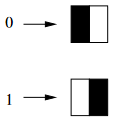
\includegraphics[scale=0.65]{Images/subpixelpattern.png}
\label{fig:subpixel}
\caption{Sub-pixel pattern to generate image share $S_1$.}
\end{figure}
Generate the other image share $S_2$ with pixels as follows: same as $S_1$ for all the white pixels of $I$, the opposite (other sub-pixel pattern) of $S_1$ for all the black pixels of $I$.

\textbf{Decrypting}

To reveal hidden image the two shares are overlayed. Each black pixel of $I$ is black in the overlay, each white pixel of $I$ is half white in overlay.
\begin{figure}[H]
\centering
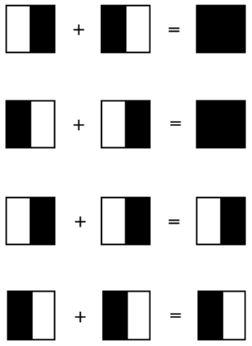
\includegraphics[scale=0.45]{Images/overlay.png}
\label{fig:subpixel}
\caption{Overlay of the two image shares.}
\end{figure}


\newpage \section{Block Ciphers}

Block ciphers are the main bulk encryption algorithms used in commercial applications.\\
Standardised block cipher AES and legacy cipher DES are widely deployed in real applications.

\subsection{Principles}

Symmetric key ciphers in which each block of plaintext is encrypted with the same key.\\
A block is a set of plaintext symbols of fixed size (typical: 64 to 256 bits).\\
Two important techniques: confusion (involves substitution to make relationship between the key and ciphertext as complex as possible) and diffusion (involves transformations that dissipate the statistical properties of the plaintext across the ciphertext). \\

\subsubsection{Product cipher}

System in which the encryption function is formed by applying (or composing) several sub-encryption functions: composition of simple functions $f_i$ for $i=1,..., r$ where each $f_i$ has a different key $K_i$.\\
$C = E(P,K) = f_r (...(f_2(f_1(P,K_1),K_2)...),K_r)$

\subsubsection{Iterated cipher}

Encryption process dividen into $r$ similar rounds. Sub-encryption functions are all the same function $g$ (round function). Each key $K_i$ is derived from overall master key $K$ using a process called key schedule.\\

\textbf{Encryption}

$W_0 = P$\\
$W_1 = g(W_0, K_1)$\\
$W_2 = g(W_1, K_2)$\\
...\\
$C = W_r = g(W_{t-1}, K_r)$.

\textbf{Decrypting}

$g$ must have inverse $g^{-1}$ with $g^{-1}(g(W,K_i)-K_i) = W$. Decryption is then the reverse of encryption:
$W_r = C$\\
$W_{r-1} = g^{-1}(W_r,K_r)$\\
$W_{r-2} = g^{-1}(W_{r-1},K_{r-1})$\\
...
$P = W_0 = g^{-1}(W_1,K_1)$\\

\subsubsection{Iterated cipher: Feistel cipher (DES)}

\textbf{Encryption}

\begin{enumerate}
    \item Split $P = W_0$ in 2 halves $W_0 = (L_0, R_0)$
    \item For each of the $r$ rounds perform: $L_i = R_{i-1}$, $R_i = L_{i-1} \oplus f(R_{i-1}, K_i)$
    \item $C = W_r$ is defined by $C = (L_r, R_r)$
\end{enumerate}

\begin{figure}[H]
\centering
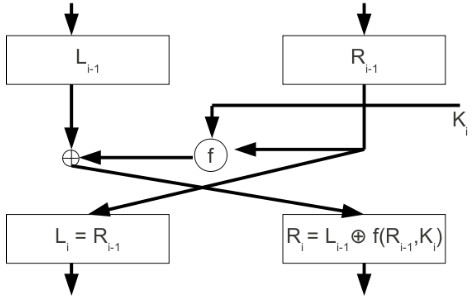
\includegraphics[scale=0.55]{Images/feistelladder.png}
\label{fig:feistelladder}
\caption{Feistel ladder diagram.}
\end{figure}

\textbf{Decryption}

\begin{enumerate}
    \item $C = (L_r, R_r)$
    \item For each of the $r$ rounds perform: $L_{i-1} = R_{i} \oplus f(L_i, K_i)$, $R_{i-1} = L_{i}$
    \item $P = (L_0, R_0)$
\end{enumerate}

We never have to invert $f$ so we can always decrypt for any function $f$. Choice of $f$ is still important as it is the only non-linear part of the encryption function.

\subsubsection{Iterated cipher: Substitution-Permutation Networks (AES)}

Block length $n$ must allow each block to be split into $m$ sub-blocks of length $l$ so that $n=lm$. 2 permutations are defined.\\
Permutation $\Pi_S$ operates on sub-blocks of size $l$ bits: $\Pi_S: \{0,1\}^l \rightarrow \{0,1\}^l$\\
Permutation $\Pi_P$ swaps the inputs from $\{1,...,n\}$: $\Pi_P: \{1,...,n\} \rightarrow \{1,...,n\}$

\textbf{Steps in SPN round function}

\begin{enumerate}
    \item Round key $K_i$ is XORd with the current state block $W_i$
    \item Each sub-block is substituted by application of $\Pi_S$
    \item Whole block is permuted using $\Pi_P$
\end{enumerate}

\begin{figure}[H]
\centering
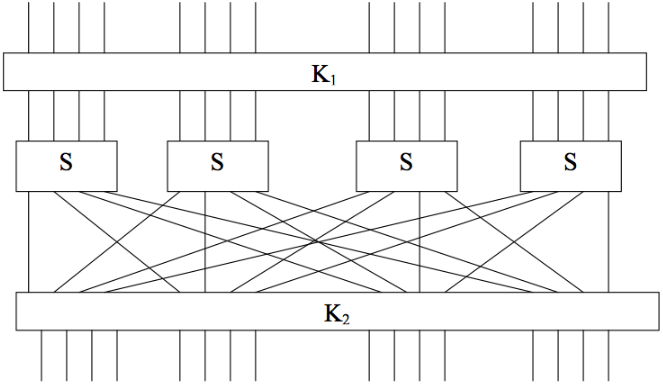
\includegraphics[scale=0.55]{Images/spnnetwork.png}
\label{fig:spnnetwoek}
\caption{SPN network.}
\end{figure}

\subsubsection{Differential and linear cryptanalysis}

Differential cryptanalysis is a chosen plaintex attack based on the idea that the difference between 2 input plaintexts can be correlated to the difference between two output cyphertexts.\\
Linear cryptanalysis is a known plaintext attack (can theoretically be used to break DES).

\subsubsection{Avalanche effects}

Good block ciphers should have avalanche effects with respect to both key and plaintext.\\
Key avalanche: small change in key (with same plaintext) should result in large change in resulting ciphertext. Shannon's notion of confusion.\\
Plaintext avalanche: small change in plaintext should result in large change in resulting ciphertext. Shannon's notion of diffusion.

\subsection{Data Encryption Standard (DES)}

DES is a 16-round Feistel cipher with key length of 56 bits and data block length of 64 bits.

\subsubsection{Encryption}

An input block of 64 bits denoted by $P$.

\begin{enumerate}
    \item The 64 bits of $P$ are permuted according to an initial fixed permutation, denoted by $IP$.
    \item 16 rounds of a Feistel operation are applied, denoted by function$f$. A different 48 bit subkey is used for each round.
    \item A final fixed inverse permutation denoted by $IP^{-1}$ is applied.
\end{enumerate}

For each round the following steps are followed:
\begin{enumerate}
    \item Expand 32 bits to 48 bits
    \item Bitwise modulo two add 48 bits to 48 bit subkey
    \item Break 48 bits into 8 blocks of 6 bits each
    \item Put block $i$ into substitution table $i$ resulting in blobk of length 4
    \item Apply permutation to resulting 32 bits
\end{enumerate}

\begin{figure}[H]
\centering
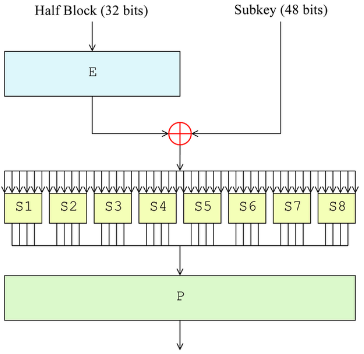
\includegraphics[scale=0.75]{Images/feistelround.png}
\label{fig:fround}
\caption{Feistel $f$ function used in DES.}
\end{figure}

\subsubsection{Key schedule}

Each of the sixteen rounds involves 48 bits of the 56 bitkey.Each 48-bit subkey is defined by a series of permutations and shifts on the full 56-bit key.

\subsubsection{Brute force attack}

A brute force attack on a block cipher consists of testing all possible $2^k$ keys in order to find the key K.\\
The right key can be identified by using a small number of ciphertext blocks, or by looking for low entropy in the decrypted plaintext.\\
In the case of DES there are $2^{56}$ keys to test so, on average, it would take $2^{55}$ trial samples to find the right key.\\
Short size of key is criticized.

\subsubsection{Double encryption}

With $K_1$ and $K_2$ two keys of the block cipher, defined by $C = E(E(P,K_1),K_2)$.\\
If key length of the original block cipher is $k$ then exhaustive key attack requires $2^{2k-1}$ trials on average.

\textbf{Meet-in-the-middle attack}

Suppose we have ciphertext/plaintext (P,C) satisfying $C = E(E(P,K_1),K_2)$.
\begin{enumerate}
    \item For each key, store $C' = E(P,K)$ in memory
    \item Check if $D(C,K')=C'$ for any key $K'$
    \item K from step 1 is $K_1$ and $K'$ from step 2 is $K_2$
    \item Check if key values in step 3 work for other (P,C) pairs
\end{enumerate}
Requires storage of one plaintext block for every possible key, a single encryption for every key and a single decryption for every key.\\
Applied to DES, this would require storage of $2^{56}$ 64-bit blocks, $2^{56}$ encryption operations and $2^{56}$ decryption operations. Expensive but much easier than brute-force search through $2^{111}$ keys.

\subsubsection{Triple encryption}

Much better security.\\
3 keys $K_1, K_2, K_3$ are used. Encryption defined by $C = E(E(E(P,K_1),K_2),K_3)$.\\
Secure from meet-in-the-middle attack.

\subsubsection{Standardised options}

\begin{enumerate}
    \item Three independent keys, the most secure. Allowed until 2023 (after that only for legacy)
    \item Two keys with $K_1 = K_3$, still secure enough (only for legacy).
    \item One key with $K_1 = K_2 = K_3$, backward-compatible but vulnerable to brute-force.
\end{enumerate}

\subsection{Advanced Encryption Standard (AES)}

Due to controversy over DES, AES was designed.\\

\subsubsection{Overview}

Symmetric block key cipher.\\
128-bit data block; 128-, 192- or 256-bit master key.\\
Number of rounds, NR, is 10, 12 or 14 (for 128-, 192-,256-bit keys).\\
Byte-based design.\\
Structure is essentially a substitution-permutation network: initial round key addition, NR-1 rounds, final round.

\subsubsection{Round transformation}

Four basic operations: ByteSub (non-linear substitution), ShiftRow (permutation), MixColumn (diffusion), AddRoundKey.\\
Essentially a SPN with $n=128$ and $l=8$.
S-box is look-up table but mathematically defined in $GF(2^8)$.

\subsubsection{Key schedule}

Master key input is 128 bits (or 192 or 256).\\
Each of the 10 (or 12 or 14) encryption/decryption rounds uses a 128-bit subkey.\\
Number of subkeys required is one for each round (10 or 12 or 14) plus an initial subkey.\\

\subsubsection{Security}

Some cracks but no significant breaks.\\
Attacks exist on reduced-round versions.\\
Related key attacks exist. Such attacks require the attacker to obtain ciphertext encrypted with a key related to the actual key in a specified way.\\
Most serious real attack so far reduces effective key size by around 2 bits.

\subsection{DES/AES comparison}

\begin{itemize}
    \item Data block size: DES: 64 bits; AES: 128 bits
    \item Key size: DES: 56 bits; AES: 128, 192 or 256 bits
    \item Design structure: DES: Feistel, bit-based; AES: SPN, byte-based, AES faster in both hardware and software
\end{itemize}

AES is the choice of today fut triple-DES is still in use in older applications.


\newpage \section{Modes of Operation and Random Numbers}

\subsection{Motivation}

\subsubsection{Why different modes ?}

Modes can provide confidentiality or authentication (and integrity) or both.\\
Some modes can be used to generate pseudo-random numbers.

\subsubsection{Importance of randomised encryption}

Problem when same plaintext block is always encrypted to same ciphertext block. \\
Randomised encryption schemes can prevent this.\\
Use of initialisation vector IV (unique or random).\\
OR: include variable state which is updated with each block.

\subsection{Features}

\begin{itemize}
    \item Efficiency: some modes allow parallel processing (while encrypting or decrypting). Some modes result in error propagation (one bit error in ciphertext results in multiple bits error in decrypted plaintext).
    \item Padding: some modes (ex. ECB, CBC) require plaintext to consist of 1+ blocks. Padding method: append single '1' and pad with enough '0' to complete the last block. Alternative: ciphertext stealing.
\end{itemize}

\subsection{Electronic Code Book (ECB) mode}

Encryption: $C_t = E(P_t, K)$. Blocks sent are $C_1, ..., C_n$.\\
Decryption: $P_t = D(C_t, K)$. Blocks received are $C_1, ..., C_n$.\\
\begin{figure}[H]
\centering
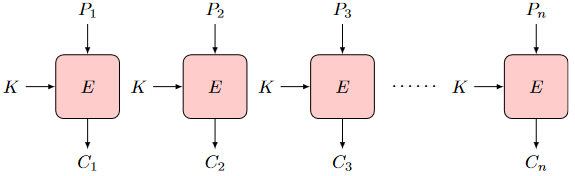
\includegraphics[scale=0.75]{Images/ecbencryption.png}
\label{fig:fround}
\caption{ECB mode encryption.}
\end{figure}
\begin{figure}[H]
\centering
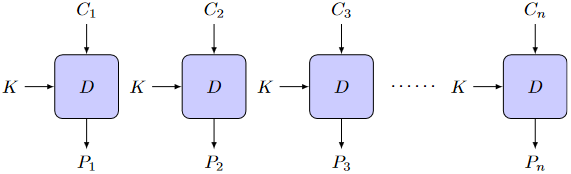
\includegraphics[scale=0.75]{Images/ecbdecryption.png}
\label{fig:fround}
\caption{ECB mode decryption.}
\end{figure}

\subsubsection{Properties}

\begin{center}
\begin{tabular}{ | c | c | } 
\hline
Randomised & no \\
\hline
Padding & Required \\ 
\hline
Error propagation & Error propagates within blocks \\ 
\hline
IV & None \\ 
\hline
Parallel encryption & Yes \\ 
\hline
Parallel decryption & Yes \\ 
\hline
\end{tabular}
\end{center}

Deterministic: not normally used for bulk encryption.

\subsubsection{Ciphertext stealing}

Suppose we want to encrypt more than one block of random bits using ECB mode with a block cipher, but without padding. This can be achieved with a technique known as ciphertext stealing.For example, suppose we encrypt a 200-bit random key using AES in ECB mode with key K.The plaintext is two blocks $M_1, M_2$ where $M_2$ is a 72-bit 'short' block.

Then we compute
\begin{center}
    $C_2 \Vert J = E(M_1, K)$\\
    $C_1 = E(M2 \Vert J, K)$
\end{center}
and send $(C_1, C_2)$ to the receiver. Here $J$ is a 56 bit random value which is never transmitted.

To decrypt we compute:
\begin{center}
    $D(C_1, K) = M_2 \Vert J$\\
    $D(C_2 \Vert J, K) = M_1$
\end{center}

\subsection{Cipher Block Chaining (CBC) mode}

Random IV is chosen and sent together with ciphertext blocks.\\
Encryption: $C_t = E(P_t \oplus C_{t-1}, K)$, where $C_0 = IV$. Blocks sent are $IV, C_1, ..., C_n$.\\
Decryption: $P_t = D(C_t, K) \oplus C_{t-1}$, where $C_0 = IV$. Blocks received are $IV, C_1, ..., C_n$.\\
\begin{figure}[H]
\centering
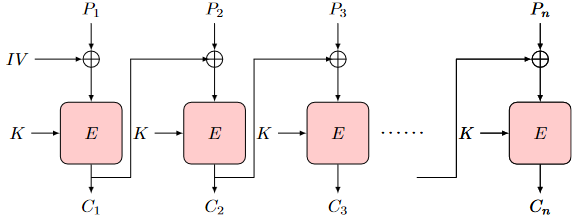
\includegraphics[scale=0.75]{Images/cbcencryption.png}
\label{fig:fround}
\caption{CBC mode encryption.}
\end{figure}
\begin{figure}[H]
\centering
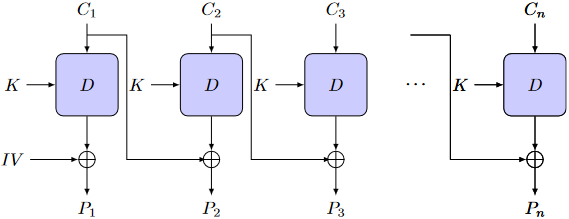
\includegraphics[scale=0.75]{Images/cbcdecryption.png}
\label{fig:fround}
\caption{CBC mode decryption.}
\end{figure}

\subsubsection{Error propagation}

\begin{figure}[H]
\centering
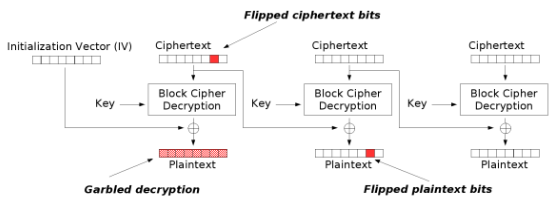
\includegraphics[scale=0.75]{Images/cbcerrorpropagation.png}
\label{fig:fround}
\caption{CBC error propagation.}
\end{figure}

\subsubsection{Properties}

\begin{center}
\begin{tabular}{ | c | p{5cm} | } 
\hline
Randomised & Yes \\
\hline
Padding & Required \\ 
\hline
Error propagation & Error propagates within blocks and into specific bits of next block \\ 
\hline
IV & Must be random \\ 
\hline
Parallel encryption & No \\ 
\hline
Parallel decryption & Yes \\ 
\hline
\end{tabular}
\end{center}

Commonly used for bulk encryption.\\
Common choice for channel protection in all versions of TLS up to TLS 1.2.

\subsection{Counter (CTR) mode}

CTR is asynchronous stream cipher. The keystream is generated by encrypting successive values of a "counter", initialised using a nonce (randomly chosen value) $N$: $O_t = E(T_t, K)$, where $T_t = N \vert \vert t$ is the concatenation of the nonce and the block number $t$.\\
Encryption: $C_t = O_t \oplus P_t$. Blocks sent are $C_1, ..., C_n$ and Nonce.\\
Decryption: $P_t = O_t \oplus C_t$. Blocks received are $C_1, ..., C_n$ and Nonce.\\

\begin{figure}[H]
\centering
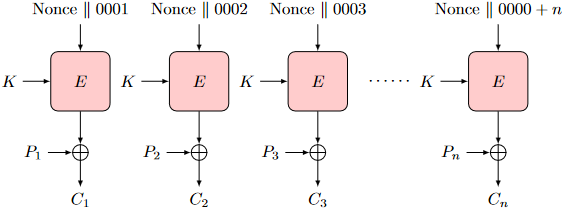
\includegraphics[scale=0.75]{Images/ctrencryption.png}
\label{fig:fround}
\caption{CTR mode encryption.}
\end{figure}
\begin{figure}[H]
\centering
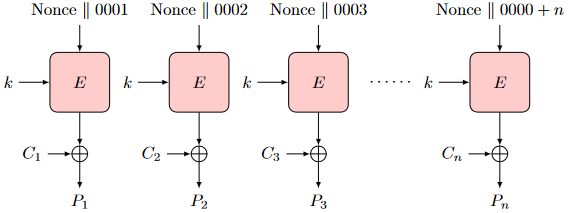
\includegraphics[scale=0.75]{Images/ctrdecryption.png}
\label{fig:fround}
\caption{CTR mode decryption.}
\end{figure}

\subsubsection{Properties}

\begin{center}
\begin{tabular}{ | c | p{5cm} | } 
\hline
Randomised & Yes \\
\hline
Padding & Not required \\ 
\hline
Error propagation & A one-bit change in the ciphertext produces a one-bit change in the plaintext at the same location \\ 
\hline
IV & Nonce must be unique \\ 
\hline
Parallel encryption & Yes \\ 
\hline
Parallel decryption & Yes \\ 
\hline
\end{tabular}
\end{center}

Synchronous stream cipher mode.\\
Good for access to specific plaintext blocks without decrypting the whole stream.\\
Basis for authenticated encryption in TLS 1.2 and TLS 1.3.

\subsection{Random Numbers}

\subsubsection{TRNG}

True Random NUmber Generator: physical process which outputs each valid string independently with equal probability.\\
Can be used to provide a seed for a PRNG.\\
Framework for design and validation of TRNG algorithms: entropy sources (physical noise source, digitization process and post-processing stages, output is any requested number of bits).

\subsubsection{PRNG}

Pseudo Random Number Generator: deterministic algorithm which approximates a TRNG.\\
Deterministic Random Bit Generators (DRBG) algorithms based on: hash functions, specific MAC (HMAC) and block ciphers in CTR mode.\\
Each generator takes seed (should be updated after some number of calls, can be generated by TRNG) as input and outputs a bit string before updating its state.

\textbf{Functions}
\begin{itemize}
    \item Instantiate: sets initial state using a seed
    \item Generate: provides output bit string
    \item Reseed: inputs new seed and updates state
    \item Test
    \item Uninstantiate: deletes state of DRBG
\end{itemize}

\textbf{Security}

\begin{itemize}
    \item Backtracking resistance: An attacker who obtains the current state of the DRBG should not be able to distinguish between the output of earlier calls to the DRBG generate function and random strings.
    \item Forward prediction resistance: An attacker who obtains the current state of the DRBG should not be able to distinguish between the output of later calls to the DRBG generate function and random strings.
\end{itemize}


\textbf{CTR\_DRBG}

Uses a block cipher in CTR mode. AES with 128-bit key is one recommended option.\\
DRBG initialised with seed (length = key length + block length, so 128+128=256bits for AES with 128-bit keys).\\
From a high entropy seed a key $K$ and state (counter) value $V$ are derived. There is no separate nonce as in normal CTR mode.\\
Counter mode encryption is then run iteratively (with no plaintext added) and the output blocks form the output

\newpage \section{Hash Functions, MAC and authenticated encryption}

Public function that:
\begin{itemize}
    \item is simple and fast to compute
    \item takes as input a message $m$ of arbitrary length and outputs a message digest $H(m)$ of fixed length
\end{itemize}

\subsection{Properties}

\begin{itemize}
    \item Collision resistant: infeasible to find $x_1, x_2$ with $H(x_1)=H(x_2)$
    \item Second-preimage resistant: given value $x_1$ it should be infeasible to find $x_2 \neq x_1$ with $H(x_1)=H(x_2)$
    \item One-way (or preimage resistant): given value $y$ it should be infeasible to find any $x$ such that $H(x)=y$
\end{itemize}
Breaking second-preimage resistance $\Rightarrow$ breaking collision resistance.

\subsection{Birthday Paradox}

In general if we choose around $\sqrt{M}$ values from a set of size $M$ the probability of getting two values the same is around 0.5.\\
Suppose hash function has output size of k bits. $2^{k/2}$ trials are enough to find a collision with probability around 0.5.\\
Today, $2^{128}$ trials is considered infeasible. To satisfy collision resistance, functions should have output of at least 256 bits.

\subsection{Iterated hash functions}

An iterated hash function splits the input into blocks of fixed size and operates on each block sequentially using the same function with fixed size inputs.\\
Merkle–Damgård construction: use a fixed-size compression function applied to multiple blocks of the message.

\subsubsection{Compression function}

Takes two $n$-bit input strings $x_1, x_2$ and produces an $n$ bit output string $y$.

\begin{figure}[H]
\centering
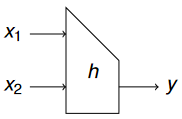
\includegraphics[scale=0.75]{Images/compressionfunction.png}
\label{fig:fround}
\caption{Compression function $h$.}
\end{figure}

\subsubsection{Merkle-Damgård construction}

\begin{enumerate}
    \item Break message $m$ into $n$-bit blocks $m_1, ..., m_l$
    \item Add padding and encoding of the length of $m$. May or may not add one block.
    \item Input each block into compression function along with chained output; use IV to get started.
\end{enumerate}

\begin{figure}[H]
\centering
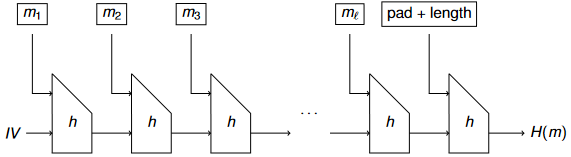
\includegraphics[scale=0.75]{Images/derklamangard.png}
\label{fig:fround}
\caption{Merkle-Damgård construction.}
\end{figure}

\subsubsection{Security}

If compression function $h$ is collision-resistant, then $H$ is sollision-resistant.\\
Some weaknesses: 
\begin{itemize}
    \item Length extension attack: once you have one collision, easy to find more.
    \item Second-preimage attacks not as hard as they should be.
    \item Collisions for multiple messages can be found without much more difficulty than collisions for 2 messages.
\end{itemize}

Many standard and former standard hash functions are Merkle-Damgård constructions: MD5, SHA-1, SHA-2 family.

\subsection{Standardized hash functions}

\subsubsection{MDx family}

MD2, MD4 and MD5.\\
Output: 128-bit.\\
All of them are broken (2006: MD5 collisions found in 1 minute on a PC).

\subsubsection{SHA-0 and SHA-1}

Based on MDx but more complex and larger output: 160-bit.\\
SHA-0 broken (collisions found in 2004).\\
SHA-1 broken (collision found in 2017).

\subsubsection{SHA-2 family}

\begin{center}
\begin{tabular}{ | c | c | c | c | } 
\hline
 & Hash size & Block size & Security match \\
\hline
SHA-224 & 224 bits & 512 bits & 2 key 3DES \\ 
\hline
SHA-512/224 & 224 bits & 1024 bits & 2 key 3DES \\ 
\hline
SHA-256 & 256 bits & 512 bits & AES-128 \\ 
\hline
SHA-512/256 & 256 bits & 1024 bits & AES-128 \\ 
\hline
SHA-384 & 384 bits & 1024 bits & AES-192 \\ 
\hline
SHA-512 & 512 bits & 1024 bits & AES-256 \\ 
\hline
\end{tabular}
\end{center}

\textbf{Padding}

Message length field is: 64 bits when block length is 512 bits; 128 bits when block length is 1024 bits.\\
Always at least one bit of padding. After the first '1', enough '0' bits are added so that after the length field is added there is an exact number of complete blocks.\\

\subsubsection{SHA-3}

MDx and SHA family are all based on the same basic design and there have been several unexpected attacks on these in recent years.\\
SHA-3 doesn’t use compression function as in Merkle–Damgård construction. Instead it uses a sponge construction.\\
Standardized in August 2015.

\subsection{Use of hash functions}

Applying hash function is NOT encryption (no key, not possible to go backwards).\\
Do not provide data authentication alone but can help achieve it: authenticate hash of message to authenticate message, building block for message authentication and signatures.

\subsubsection{Storing passwords}

Usual to store user passwords on servers using hash functions.\\
Store salted hashes of passwords: pick random $salt$, compute $h=H(pw, salt)$, store $(salt,h)$.\\
Easy to check entered password, hard to recover $pw$ from $h$. Attacker needs to store a different dictionary for each $salt$.\\
Using slower hash function slows down password guessing.

\subsection{Message Authentication Code (MAC)}

Cryptographic mechanism used for message integrity and authentication.\\
On input a secret key $K$ and an arbitrary length message $M$, a MAC algorithm outputs a fixed-length tag: $T=MAC(M,K)$.\\
Symmetric key algorithm: sender and receiver both have secret key $K$.\\
Sender sends pair $(M,T)$ but $M$ may or may not be encrypted.\\
Recipient recomputes tag $T' = MAC(M', K)$ on received message $M'$ and check $T'=T$.

\subsubsection{Properties}

\begin{itemize}
    \item Unforgeability: not feasible to produce $M$ and $T$ such that $T=MAC(M,K)$ without knowledge of $K$
    \item Unforgeability under chosen message attack: attacker is given access to forging oracle (on input any message $M$ of the attacker's choice the MAC tag $T=MAC(M,K)$ is returned). It is not feasible for the attacker to produce a valid $(M,T)$ pair that was not already asked to the oracle.
\end{itemize} 

\subsubsection{HMAC}

Built from any iterated cryptographic hash function $H4$, e.g.,MD5, SHA-1, SHA-256, ...\\
Standardized and used in many applications including TLS and IPsec.

\textbf{Construction}

$HMAC(M,K) = H((K \oplus opad) \Vert H (( K \oplus ipad) \Vert M))$ where $M$ = message to be authenticated, $K$ = key padded with zeros to the block size of $H$, $opad$ = fixed string 0x5c5c5c...5c, $ipad$ = fixed string 0x363636...36, $\Vert$ denotes concatenation of bit strings.

\textbf{Security}

Secure if $H$ is collision-resistant or pseudo-random.\\
Designed to resist length extension attacks (even of $H$ is Merkle-Damgård hash function).\\
Often used as pseudorandom function for deriving keys in cryptographic protocols.

\subsubsection{Authenticated encryption}

Alice and Bob have shared key K. Alice has message $M$ she wants to send to Bob with confidentiality and authenticity/integrity.\\
2 options: split $K$ in 2 parts, encrypt with $K_1$ and use $K_2$ with a MAC; use dedicated algorithm which provides both properties (authenticated encryption).

\textbf{Combining encryption and authentication}

\begin{itemize}
    \item encrypt and MAC: encrypt $M$, apply MAC to $M$ and send two results.
    \item MAC then encrypt: apply MAC to $M$ to get tag $T$ then encrypt $M \Vert T$ and send ciphertext
    \item encrypt then MAC: encrypt $M$ to get ciphertext $C$ then MAC $C$ and send 2 $C \Vert T$.
\end{itemize}

Encrypt-then-MAC is the safest approach.

\textbf{Authenticated encryption with associated data (AEAD)}

AEAD algorithm: symmetric key cryptosystem.\\
Inputs: message $M$, associated data $A$, shared key $K$.\\
Output $O$ may contain different elements such as ciphertext and tag. Sender sends $O$ and $A$ to recipient.\\
Receiver outputs either a message $M$ or reports fail.\\
Any AEAD algorithm should provide confidentiality for $M$ and authentication for both $M$ and $A$.

\subsubsection{Galois counter Mode (GCM)}

Block cipher mode providing AEAD.\\
Most commonly used mode in TLS.\\
Combines CTR mode on a block-cipher (tipically AES) with a special keyed hash function GHASH.\\
GCM using AES can be faster than using AES with HMAC.

\textbf{GCM algorithm}

GHASH uses multiplication in finite field $GF(2^{128})$.\\
Inputs: plaintext $P$, authenticated data $A$ and nonce $N$.\\
Values $u$ and $v$ are minimum number of 0s required to expand $A$ and $C$ to complete blocks.\\
Outputs: ciphertext $C$ and tag $T$. (length of $A$, $len_A$ and length of $C$, $len_C$ are 64-bit values).\\
TLS: length of $T$ is $t=128$ bits and $N$ is 96 bits. Initial block input to CTR mode of E (CTR in diagram) is $J_0 = N \Vert 0^31 \Vert 1$.\\
$inc_{32}$ increments the right-most 32 bits of the input string by 1 modulo $2^{32}$.

\begin{figure}[H]
\centering
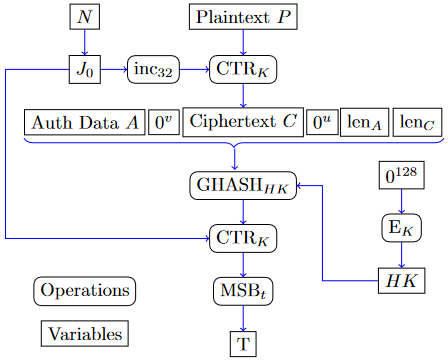
\includegraphics[scale=0.75]{Images/gcmalgorithm.png}
\label{fig:fround}
\caption{GCM algorithm.}
\end{figure}

\begin{figure}[H]
\centering
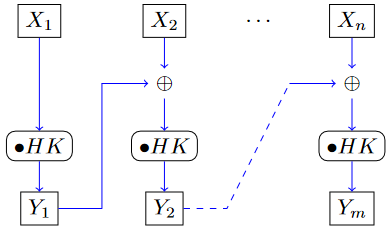
\includegraphics[scale=0.75]{Images/ghash.png}
\label{fig:fround}
\caption{GHASH.}
\end{figure}

For GHASH: output is $Y_m=GHASH_{HK} (X_1,...,X_m)$, $\bullet$ is multiplication in $GF(2^{128})$, $HK=E(0^128,K)$ is the hash subkey.

\textbf{GCM decryption}

The elements transmitted to the receiver are the ciphertext $C$, the nonce $N$, the tag $T$ and the authenticated data $A$.\\
All elements required to recompute the tag $T$ are available to the receiver who shares key $K$. The tag is recomputed and checked with received tag. If tags do not match then output is declared invalid.\\
If the tag is correct then the plaintext can be recomputed by generating the same key stream, from CTR mode, as is used for encryption.


\newpage \section{Number Theory for Public Key Cryptography}

\subsection{Chinese remainder theorem}

Let $d_1,..., d_r$ be pairwise relatively prime and $n= d_1 ... d_r$. Given any interegers $c_i$ there exists a unique integer $0 \leq x < n$ such that $x=c_i$ mod $d_i$ for all $i \leq r$.\\
In fact $x = \sum (\frac{n}{d_i})y_i c_i$ mod $n$ where $y_i = (\frac{n}{d_i})^{-1}$ mod $d_i$.

\subsubsection{Example}

Solve $x = 5$ mod 6, $x=33$ mod 35.\\
6 and 35 are relatively prime so we can use CRT. Set $n = 6*35=210$.\\
$\frac{210}{6}y_1 = 1$ mod 6, 
$\frac{210}{35}y_2 = 1$ mod 35\\
$35 y_1 = 1$ mod 6, 
$6 y_2 = 1$ mod 35\\ 
$y_1 = 5$ mod 6, 
$y_2 = 6$ mod 35\\ 
$x = \sum (\frac{n}{d_i})y_i c_i$ mod n\\
$x = (35*5*5)+(6*6*33)$ mod 210\\
$x = 173$ mod 210\\

\subsection{Euler function $\phi$}

For a positive integer $n$, the Euler function $\phi (n)$ denotes the number of positive integers less than $n$ and relatively prime to $n$.\\
The set of positive integers less than $n$ and relatively prime to $n$ form the reduced residue class $\mathbb{Z}^*_n$.

\subsubsection{Properties}

\begin{itemize}
    \item $\phi (p) = p-1$ for $p$ prime
    \item $\phi (pq) = (p-1)(q-1)$ for $p$ and $q$ distinct primes.
    \item Let $n = p_1^{e_1}...p_t^{e_t}$ where $p_i$ are distinct primes. Then $\phi (n) = \prod p_i^{e_i -1} (p_i -1)$.
\end{itemize}

\subsubsection{Theorems}

\begin{itemize}
    \item Fermat: Let $n$ be prime. Then $a^{p-1} = 1$ mod $p$ for all integers $1 < a < p-1$.
    \item Euler: $a^{\phi(n)} = 1$ mod $n$ if $gcd(a,n) = 1$.
\end{itemize}

\subsection{Testing for primality}

Methods used in practice are probabilistic.

\subsubsection{Fermat primality test}

If we examine $n$ and find that $a^{n-1} \neq 1$ mod $n$ then we know $n$ is not prime.\\
We reduce failure probability by repeating test with different base values $a$.\\

Inputs: $n$ = number to test; $k$ = parameter determining number of times to test for primality.\\
Output: 'composite' if $n$ is composite, otherwise 'probable prime'.\\

\textbf{Effectiveness}

If the tests outputs 'composite' then $n$ is definitely composite. If the test outputs 'probable prime', $n$ is said to be pseudoprime.\\
Carmichael numbers: the tet will always output 'probable prime' for every $a$ with $gcd(a,n) = 1$ (561, 1105, 1729, 2465, ...).

\subsubsection{Miller-Rabin test}

Same idea as Fermat test. \\
Guaranteed to detect composites if run sufficiently many times.\\
Most widely used to generate large prime numbers.

\textbf{Square roots of 1}

Modular square root of 1 is a number $x$ with $x^2 = 1$ mod $n$.\\
When $n=pq$ there are 4 square roots of 1. Two of these are 1 and -1 (trivial roots). The 2 others are the non-trivial roots.\\
If $x$ is a non-trivial square root of 1 then $gcd(x-1,n)$ is a non-trivial fator of $n$. Existence of non-trivial square root implies that $n$ is composite.

\textbf{Algorithm}

Assume $n$ is odd. Define $u,v$ such that $n-1=2^v u$ where $u$ is odd.
\begin{enumerate}
    \item Pick $1 < a < n-1$ randomly.
    \item $b = a^u$ mod $n$
    \item If b == 1 then return 'probable prime'
    \item For $j = 0$ to $v-1$
    \begin{itemize}
        \item If b == -1 return 'probable prime'
        \item Else set $b=b^2$ mod $n$
    \end{itemize}
    \item Return 'composite'
\end{enumerate}

\textbf{Effectiveness}

If the test returns 'composite', $n$ is composite.\\
If the test returns 'probable prime', $n$ may be composite.\\
If $n$ is composite the test returns 'probable prime' with probability 1/4.\\
Therefore we repeat algorithm $k$ times while output is 'probable prime'.\\
The k-times algorithm will output 'probable prime' when $n$ is composite with probability no more than $(1/4)^k$.\\
No composites less than 341,550,071,728,321 which pass the test for the seven bases $a=2,3,5,7,11,13,17$.

\textbf{Generating large primes}\label{Generating large primes}

\begin{enumerate}
    \item Choose random odd integer $r$ of the same number of bits as the required prime.
    \item Test if $r$ is divisible by any of a list of small primes.
    \item Apply Miller-Rabin test with 5 (random or fixed) bases.
    \item If $r$ fails any test then set $r := r+2$ and return to step 2. (to have completely random primes start again at step 1)
\end{enumerate}

\subsection{Complexity theory}

\subsubsection{Definitions}

The computational complexity of an algorithm is measured by its time and space requirements as functions of the size of the input $m$.\\
We say $f(m) = \mathcal{O} (g(m))$ if there exist constants $c>0$ and $m_0$ such that $f(m) \leq c * g(m)$ for $m\geq m_0$.\\\\
Polynomial time function: $f(m)=\mathcal{O} (m^t)$ where $t > 0$.\\
Exponential time function: $f(m)=\mathcal{O} (b^m)$ where $b > 1$. Brute-force key search is exponential.\\

\subsubsection{Integer factorisation}

Given an integer, find its prime factor.\\
Factorisation by trial division is an exponential time algorithm and is hopeless for numbers of a few hundred bits.\\
Best current method: number field sieve (sub-exponential: better than exponential but worse than polynomial).

\subsubsection{Discrete logarithm problem (DLP)}

Let $\mathbb{G}$ be a cyclic group with generator $g$. The DEL in $\mathbb{G}$ is given $y \in \mathbb{G}$, find $x$ such that $y=g^x$.\\
Best method for solving DLP in $\mathbb{Z}_p^*$: variant of number field sieve (sub-exponential).\\
DLP can also be defined on elliptic curve groups (see later): best algorithms are exponential.

\newpage \section{Public Key Cryptography and RSA}

\subsection{Public Key Cryptography (PKC)}

Public key cryptography is another name for asymmetric cryptography.\\
The encryption and decryption keys are different.\\
The encryption key is a public key which can be known to anybody.\\
The decryption key is a private key which should be known only to the owner of the key.\\
Finding the private key from knowledge of the public key must be a hard computational problem.

\subsubsection{One-way functions}

$f$ is a one-way function if it is easy to compute $f(x)$ given $x$ but it is hard to compute $f^{-1}(y)=x$ given $y$.\\
Two functions believed to be one-way functions:
\begin{itemize}
    \item Multiplication of large primes: inverse function is integer factorisation
    \item Exponentiation: inverse function is taking discrete logarithms
\end{itemize}

\subsubsection{Trapdoor one-way functions}

One-way function such that given additional information (the trapdoor) it is easy to compute $f^{-1}$.\\
Example: modular squaring.\\
Let $n=pq$ be the product of two large prime numbers $p$ and $q$ and define $f(x)=x^2$ mod $n$. Trapdoor is factorisation of $n$ - knowledge of $p$ and $q$ gives an efficient algorithm to find square roots (add exercise here).

\subsubsection{Why PKC ?}

Two advantages:
\begin{itemize}
    \item Key management is simplified: key do not need to be transported confidentially.
    \item Digital signatures can be obtained.
\end{itemize}

\subsubsection{Using PKC}

Each user $A$ stores her public key in public directory. Anyone can obtain that key and use it to form an encrypted message for $A$.\\
Since only $A$ has the private key, only $A$ can decrypt and recover the message.

\subsection{RSA}

\subsubsection{RSA key generation}

\begin{enumerate}
    \item Let $p, q$ be distinct primes randomly chosen from the set of all primes of a certain size.
    \item $n = pq$
    \item Select $e$ randomly with $gcd(e,\phi(n))=1$
    \item $d = e^{-1}$ mod $\phi(n)$
    \item Public key is the pair $n$ and $e$
    \item Private key consists of values $p$, $q$ and $d$.
\end{enumerate}

\subsubsection{RSA operations}

\textbf{Encryption}

Public key is $K_E = (n,e)$.\\
Input: any value $0 < M < n$. Any message needs to be pre-processed (includes coding as a number and adding randomness - see later)\\
Compute $C=E(M,K_E)=M^e$ mod $n$.

\textbf{Decryption}

Private key for decryption is $K_D=d$.\\
Compute $D(C,K_D)=C^d$ mod $n=M$.

\textbf{Example}

\begin{itemize}
    \item Key generation: Suppose $p=43, q=59$. Then $n=pq=2537$ and $\phi(n)=(p-1)(q-1)=2436$.\\
    Choose $e=5$ then $d=e^{-1}$ mod $\phi(n)=5^{-1}$ mod $2436 = 1949$.
    \item Encryption: $M = 50 \Rightarrow C = M^5 $mod $2537 = 2488$.
    \item Decryption: $M = C^{1949}$ mod $2537 = 50$.
\end{itemize}

\subsubsection{Correctness of RSA encryption}

We need to know that encryption followed by decryption gets back where we started from: $(M^e)^d$ mod $n = M$.

\newpage \section{RSA: Implementation and Security}

\subsection{Implementing RSA}

\subsubsection{Generating $p$ and $q$}

Should be random primes of chosen length (today: usually 1536 bits).\\
Use of the Miller-Rabin test to generate random prime (see \ref{Generating large primes}). 

\textbf{Are there enough prime numbers ?}

Prime number theorem: primes thin out as the numbers get larger.\\
$\pi(x)$ = nb of primes less than $x$. $\pi(x)/(\frac{x}{ln(x)}) \longrightarrow 1 $. So proportion of primes up to $x$ is about $ln(x)$.\\
Well over $2^{1500}$ 1536-bit primes: brute-force searching impossible.

\subsubsection{Selecting $e$}

Should be random for max security.\\
Usually small value for efficiency.\\
$e=3$ is the smqllest vqlue qnd is sometimes used but not very secure, $e=2^{16}+1$ is a popular choice.\\
A smaller than average $d$ value is also possible. However, to avoid known attacks $d$ should be at least $\sqrt{n}$.

\subsubsection{Fast exponentiation: square-and-multiply}

Exponent $e$ writen in binary: $e=e_0 2^0 + e_1 2^1 + ... + e_k 2^k$ where $e_i$ are bits.\\

\begin{figure}[H]
\centering
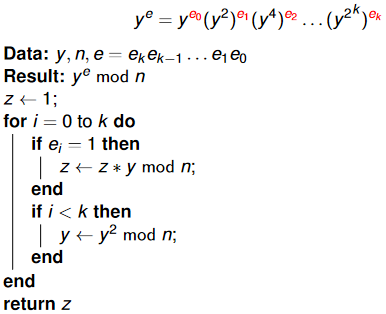
\includegraphics[scale=0.65]{Images/squareandmultiply.png}
\label{fig:fround}
\caption{Square-and-multiply algorithm.}
\end{figure}

\textbf{Cost}

If $2^k \leq e < 2^{k+1}$ then the algorithm uses $k$ squarings.\\
If $b$ of the $e_i$ bits are 1 then the algorithm uses $b-1$ multiplications.\\
If $n$ is 3072-bit RSA modulus: private exponent $d$ is length at most 3072 bits, and computing $M^d$ mod $n$ requires at most 3072 modular squarings and 3072 modular multiplications (on average half of the bits of $d$ are '1's so only 1536 multiplications are needed).

\subsubsection{Faster decryption with CRT}

First compute $M_p = C^{d mod p-1}$ mod $p$, $M_q = C^{d mod q-1}$ mod $q$.\\
Solve for $M$ mod $n$ using CRT: $M=M_p$ mod $p$, $M=M_q$ mod $q$.\\
$M = q * (q^{-1} mod p) * M_p + p * (p^{-1} mod q ) * M_q$ mod $n$.

\textbf{Example}

$n=43*59=2537$. Ciphertext $C=2488$. Decryption exponent $d=1949$.\\
$d$ mod $p-1 = 1949$ mod $42 = 17$\\
$d$ mod $q-1 = 1949$ mod $58 = 35$\\
$M_p = 2488^{17}$ mod $43 = 7$\\
$M_q = 2488^{35}$ mod $59 = 50$\\
Using CRT solution is $M=50$.

\textbf{How much faster ?}

Exponents (d mod p-1) and (d mod q-1) are about half the length of $d$.\\
Complexity of exponentiation increases with cube of input length $\Rightarrow$ computing $M_p$ and $M_q$ each use 1/8 the computation of $M=C^d $ mod $n$. Can be done in parallel to be 8 times faster.\\
Good idea to store $p$ and $q$ with private exponent $d$.

\subsubsection{RSA padding}

Using RSA directly on messages encoded as numbers is vulnerable to :
\begin{itemize}
    \item building up dictionary of known plaintexts
    \item guessing plaintext and checking to see if it encrypts to the ciphertext
    \item Håstad's attack (see \ref{Håstad's attack})
\end{itemize}
Padding mechanisms must be used to prepare messages for encryption: must include redundancy and randomness.

RSA is often used for hybrid encryption:
\begin{enumerate}
    \item Encrypt random value $r$ using RSA public key.
    \item Use $r$ (after hashing) as the key in a symmetric-key encryption algorithm.
\end{enumerate}

\textbf{PKCS Number 1}

Encryption block format is:
\begin{center}
\begin{tabular}{ | c | c | c | c | c | } 
\hline
00 & 02 & $PS$ & 00 & $M$ \\
\hline
\end{tabular}
\end{center}
where 00 and 02 are bytes, $PS$ is a pseudo-random string on nonzero bytes (minimum 8 bytes) and $M$ is the data to be encrypted.\\
The length of the block is the same as the length of the modulus.\\
The byte 02 and padding ensure that even short messages result in a large integer value for encryption.

\textbf{Optimal Asymmetric Encryption Padding (OAEP)}

Has security proof in a suitable model.\\
Encoded message uses a $k$-bit random value $r$ and a $k$-bit constant $d$. Typical value for $k$ is 256.\\
The data to be encrypted $m$ is padded with at least one byte to make $\vert n \vert - 2k-8$ bits where $\vert n \vert$ = nb of bits in the RSA modulus $n$.\\
Two random hash functions G and H are used, derived from SHA-256.\\
Encoding algorithm, can be easily inverted without any secret.

\begin{figure}[H]
\centering
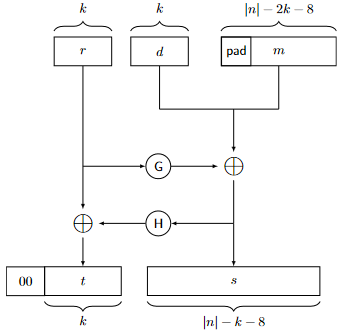
\includegraphics[scale=0.7]{Images/oaepencoding.png}
\label{fig:fround}
\caption{OAEP encoding.}
\end{figure}

\subsubsection{Håstad's attack}\label{Håstad's attack}

Suppose the same message is encrypted without padding to three different recipients.\\
Suppose the public exponent $e=3$ is used by all recipients.\\
The cryptanalyst has 3 ciphertexts $C_1 = M^3$ mod $n_1$, $C_2 = M^3$ mod $n_2$ and $C_3 = M^3$ mod $n_3$.\\
These equations can be solved by the CRT to obtain $M^3$ in the ordinary (non-modular) integers. Then $M$ can be found by taking a cube root.

\subsection{Security of RSA}

\subsubsection{Factorisation}

An adversary who can factorise $n$ into its prime factors $p$ and $q$ can recover private key $d$ and reveal all messages.\\
Breaking RSA is not harder than the factorisation problem, it is unknown if it is as hard (also unknown whether factorisation is really computationally hard).

Theorem (Miller): determining $d$ from $e$ and $n$ is as hard as factorising $n$.

\textbf{Miller's algorithm}

\begin{enumerate}
    \item Define $u,v$ such that $ed-1=2^v u$ where $u$ is odd.
    \item Consider sequence $a^u, a^{2u}, ..., a^{2^{v-1}u}, a^{2^{v}u}$ mod $n$.
    \item Notice tha $a^{2^vu}=a^{ed-1}=a^{ed}a^{-1}=aa^{-1}=1$ mod $n$ so there is a square root of 1 somewhere in his sequence.
    \item With probability at least 0.5 the sequence contains a non-trivial square root of 1 modulo $n$ thereby revealing the factors of $n$
    \item If not, choose a new $a$ and repeat.
\end{enumerate}

\textbf{Quantum computers}

Shor's algorithm can factorise in polynomial time on a quantum computer.\\
NIST is running open competition to standardise public key cryptography secure against quantum computers.

\subsubsection{Side Channel Attacks on RSA}

First made public in 1996 by Paul Kocher.\\
Also apply to most other public and symmetric key cryptosystems.\\
Many different kinds of side-channels are known including timing attacks, power analysis, and fault analysis.

Timing attacks: attacker measures distribution of timing of $a \cdot b$ mod $n$ on target platform.

\textbf{Timing attack on square-and-multiply}

Recall that square-and-multiply performs for each exponent bit $e_i$ either: a squaring only when $e_i=0$; or a squaring and a multiplication when $e_i=1$.\\
Measure correlations between the known distribution and the actual time used for different input.\\
Find each bit $e_i$ of the private exponent before moving to the next.

\textbf{Timing attack on CRT}

When the Chinese Remainder Theorem is used, a timing attack can be used to find one factor of $n$, say $p$.\\
Choose different input $C$ values to change the timing of modular reduction $C$ mod $p$.\\
If $C_1$ and $C_2$ cause different timings then there is probably a multiple of $p$ between them.\\
A binary search can be used to find $p$ and then $n$ can be factorised.

\textbf{Countermeasures}

Usually degrade performance.\\
\begin{itemize}
    \item Computing in constant time - run 'dummy' multiplication when $e_i = 0$ in square-and-multiply algorithm
    \item Montgomery ladder - makes every operation depend on the key to avoid some default attacks
    \item Randomising RSA message, which can hide either which value is actually multiplied by exponent bit in square-and-multiply algorithm; or size of value used in CTR modular reduction.
\end{itemize}

\subsubsection{Summary}

\begin{itemize}
    \item Factorisation of the modulus is the best known attackagainst RSA in the case that standardised padding is used
    \item Finding the private key from the public key alone is as hard as factorising the modulus
    \item It is an open problem whether there is any way of breaking RSA encryption without factorising the modulus
    \item Side channels are an important threat to consider
\end{itemize} 

\newpage \section{Public Key Cryptosystems based on Discrete Logarithms}

\subsection{Diffie-Hellman Key Exchange}

\subsubsection{Protocol}

Alice and Bob want to share a secret using only public communications.\\
Public knowledge: generator $g$ of a multiplicative group $G$ of order $t$ (originally $\mathbb{Z}_p^*$ for large $p$, now elliptic curve group).\\
Alice and Bob each select random values $a$ and $b$ where $0<a,b<t$.\\
Alice sends $g^a$ to Bob (insecure channel).\\
Bob sends $g^b$ to Alice (insecure channel).\\
Alice and Bob both compute secret key $Z=g^{ab}$. $Z$ can be used to compute a key for $AES$ for example (using key derivation function based on a public hash function).

\begin{figure}[H]
\centering
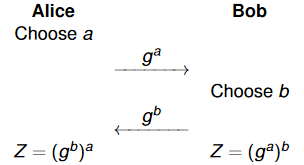
\includegraphics[scale=0.7]{Images/diffiehellmanprotocol.png}
\label{fig:fround}
\caption{Diffie-Hellman protocol.}
\end{figure}

\subsubsection{Properties}

\textbf{Security}

An attacker who can find discrete logarithms in $G$ can break the protocol: intercept $g^a$ and take discrete log to find $a$, then compute $g^{ab}$ in the same way as Bob.\\
Unknown whether there is better way to break the protocol.\\
Diffie-Hellman problem: find $Z=g^{ab}$ from knowledge of $g^a$ and $g^b$.

\textbf{Authenticated Diffie-Hellman}

In the basic Diffie–Hellman protocol the messages between Alice and Bob are not authenticated.\\
Neither Alice nor Bob knows who the secret $Z$ is shared with unless the messages are authenticated.\\
This allows a man-in-the-middle attack, where the adversary sets up two keys, one with Alice and one with Bob, and relays messages between the two.\\
Authentication can be added in different ways, for example by adding digital signatures (see next section).

\textbf{Static and ephemeral Diffie-Hellman}

The protocol above uses ephemeral keys: used once and then discarded.\\
Static D-H: Alice chooses long-term private key $x_A$ with corresponding public key $y_A=g^{x_A}$. Bob does the same with $x_b$ and $y_B$. Now Alice and Bob can find a shared secret $S=g^{x_A x_B}$ just by looking up (or knowing) each others' public keys. $S$ is static: it stays the same long-term until Alice and Bob change their public keys.

\subsection{Elgamal cryptosystem}

\subsubsection{Algorithm}

\textbf{Key generation}

\begin{itemize}
    \item Select prime $p$ and a generator $g$ of $\mathbb{Z}_p^*$
    \item Select long term private key $0<x<p-1$
    \item $y= g^x$ mod $p$
    \item Public key is $(p,g,y)$
    \item Often $p$ and $g$ are shared between all users in some system.
\end{itemize}

\textbf{Encryption}

Public key is $K_E = (p,g,y)$.
\begin{enumerate}
    \item For any value $0<M<p$
    \item Choose $k$ at random and compute $g^k$ mod $p$
    \item $C=E(M,K_E)=(g^k$ mod $p, My^k$ mod $p)$
\end{enumerate}

\textbf{Decryption}

Private key is $K_D=x$ with $y=g^x$ mod $p$
\begin{enumerate}
    \item $C=(C_1,C_2)$
    \item Compute $C_1^x$ mod $p$
    \item $D(C, K_D) = C_2 \cdot (C_1^x)^{-1}$ mod $p = M$.
\end{enumerate}

\textbf{Example}

\begin{enumerate}
    \item Key generation: Choose prime $p=181$ and generator $g=2$.\\
    Private key of $A$ is $x=50$.\\
    Public key is $p=181, g=2, y=116$.\\
    \item Encryption: Sender wants to send $M = 97$.\\
    Sender chooses random $k = 31$.\\
    Ciphertext is $(98,173)=(C_1, C_2)$.
    \item Decryption: $A$ receives $(C_1, C_2)$ and recovers $M$ by:\\
    $C_1^x = 98^{50}$ mod $p = 138$.\\
    $M = C_2 * (C_1^x)^{-1}$ mod $p = 97$.
\end{enumerate}

\subsubsection{Security}

If an attacker can solve the discrete log problem, the system can be broken by determining the private key $x$ from $g^x$ mod $p$.\\
Possible for many users to share the same $p$ and $g$ values.\\
No need for padding as in RSA - each ciphertext is already randomised.

\subsection{Elliptic curves}

Algebraic structures formed from cubuc equations.\\
Example: set of all $(x,y)$ which satisfy $y^2= x^3+ax+b$ mod $p$. This is a curve over the field $\mathbb{Z}_p$ but elliptic curves can be defined over any field.\\
Once an identity element is added, a binary operation can be defined on these points. With this operation the elliptic curve points form an elliptic curve group.

\subsubsection{Choosing elliptic curves}

Standard application usually use standard curves.\\
Example: NIST curve P-192.

\subsubsection{Discrete logarithms on elliptic curves}

The discrete logarithm can be defined on elliptic curves groups - if we denote the elliptic curve operation as multiplication then the definition is the same as in $\mathbb{Z}_p^*$.\\
Best known algorithms to solve elliptic curve discrete log problem: exponential. Consequently elliptic curve implementations use much smaller keys.\\
Compared with RSA the relative advantage of elliptic curve cryptography will increase at higher security levels.

\subsubsection{Elliptic curve cryptography}

\begin{table}[H]
\begin{center}
\begin{tabular}{ | p{3.5cm} | p{3.5cm} | p{3.5cm} | }
\hline
Symmetric key length  & RSA modulus length or length of $p$ in $\mathbb{Z}_p^*$ & Elliptic curve group size \\
\hline
80 & 1024 & 160\\
\hline
128 & 3072 & 256\\
\hline
192 & 7680 & 384\\
\hline
256 & 15360 & 512\\
\hline
\end{tabular}
\caption{Comparing strength of elliptic curve cryptography.}
\end{center}
\end{table}

Brute force search of 128-bit key for AES takes roughly same computational effort as for taking discrete logarithms in $\mathbb{Z}_p^*$ with $p$ of 3072-bits or on an elliptic curve with elements of size 256 bits.

Most cryptosystems based on discrete logarithms can be constructed with elliptic curves as well as in $\mathbb{Z}_p^*$: Diffie-Hellman and Elgamal for example.

\subsection{Post-quantum cryptography}

Most public key cryptography is use today will be broken if quantum computers become available due to Shor’s algorithm for factorisation, which can also be used to find discrete logarithms.\\
Symmetric key cryptography can still be used but with double length keys due to Grover’s algorithm for searching.\\
Currently no post-quantum replacement for Diffie-Hellman: promising candidate is the use of isogenies on elliptic curves.

\newpage \section{Digital Signatures and Certificates}

\subsection{Properties}

\subsubsection{Confidentiality and authentication}

Message AUthentication Codes (MACs) allow only ean entity with the shared secret to generate a valid MAC tag, providing data integrity and data authentication.\\
Digital signatures use public key cryptography to provide the properties of a MAC and more: only the owner of the private key can generate a correct digital signature.\\

\subsubsection{Comparison to physical signatures}

\begin{center}
\begin{tabular}{ | c | c | }
\hline
Physical signatures & Digital signatures \\
\hline
Produced by human & Produced by machine \\
\hline
Same on all the documents & Function of message\\
\hline
Easy to recognize & Requires computer to check\\
\hline
\end{tabular}
\end{center}

Both need to be difficult to forge.

\subsubsection{Elements}

Digital signature scheme has 3 algorithms: key generation, signature generation, signature verification.\\
Key generation outputs 2 keys: private signature generation key (or signing key) $K_S$; and a public signature verification key $K_V$.

\subsubsection{Signature generation}

Alice wishes to generate signature on message $m$.\\
Inputs: Alice's private signing key $K_S$ and the message $m$.\\
Output: signature $\sigma = Sig(m, K_S)$.\\
Only the owner of $K_S$ should be able to generate a valid signature.

\subsubsection{Signature verification}

Bob wishes to verify a claimed signature $\sigma$ on the message $m$.\\
Inputs: Alice's public verification key $K_V$, the message $m$ and the claimed signature $\sigma$.\\
Output: boolean $Ver(m,\sigma,K_V)$.\\
Anyone should be able to use $K_V$ to verify a signature.

\textbf{Required properties}

Correctness: $\sigma = Sig(m,K_S) \Rightarrow Ver(m,\sigma,K_V) = $true.\\
Unforgeability: computationally infeasible for anyone without $K_S$ to construct $m$ and $\sigma$ such that $Ver(m,\sigma,K_V) = $true.\\
Sig may be randomised so there are many possible signatures for a single message.\\
Stronger security definition: assume attacker has access to a chosen message oracle (forging (new) signature should be difficult even with access to signatures on chosen messages).

\subsubsection{Security goals}

Attacks:
\begin{itemize}
    \item Key recovery: attacker attempts to recover $K_S$ from $K_V$ and some known signatures.
    \item Selective forgery: attacker chooses message and attempts to obtain a signature on that message.
    \item Existential forgery: attacker attempts to forge signature on any message not previously signed.
\end{itemize}
Modern digital signatures are considered secure only if they can resist existential forgery under a chosen message attack.

\subsection{RSA Signatures}

\subsubsection{Key generation}

Generated in the same way as RSA encryption keys.
\begin{itemize}
    \item Modulus $n=pq$ is computed from random large primes $p$ and $q$
    \item Two exponents $e$ and $d$ are generated with $ed$ mod $\phi(n) = 1$
    \item Private signing key is $K_S = (d,p,q)$
    \item Public verification key is $K_S = (e,n)$
    \item A hash function $h$ is also required and should be a fixed public parameter of the signature scheme.
\end{itemize}

\subsubsection{Operations: signature generation and verification}

Generation: inputs are the message $m$, the modulus $n$ and the private exponent $d$.\\
1. Compute signature $\sigma = h(m)^d$ mod $n$.

Verification: inputs are the message $m$, the claimed signature $\sigma$ and the public key $(e,n)$.\\
1. Compute $h' = h(m).$\\
2. Check if $\sigma^e$ mod $n = h'$ and if so output true, else false.

\subsubsection{Hash functions for RSA signatures}

Following 2 choices can be proven secure with suitable assumptions:
\begin{itemize}
    \item Full domain hash: implementation of $h$ which can take values randomly in the range 1 to $n$.
    \item PSS: probabilistic hashing function similar to OAEP used for RSA encryption and is standardised in the PKCS #1 standard.
\end{itemize}

\subsection{Discrete Logarithm Signatures}

Rely on the difficulty of the discrete log problem.

\subsubsection{Elgamal in $\mathbb{Z}_p^*$}

\textbf{Key genration}

Let $p$ be a large prime with generator $g$. Private signing key is $0 < x < p-1$.\\
Public verification key: $y = g^x$ mod $p$. Values $p, g, y$ are public knowledge.

\textbf{Signature generation}

To sign message $m$ with signing key $x$:
\begin{itemize}
    \item Select random $0<k<p-1$ and compute $r = g^^k$ mod $p$
    \item Compute $s = k^{-1}(m-xr)$ mod $(p-1)$
    \item Signature is $\sigma = (r,s)$
\end{itemize}

\textbf{Signature verification}

Given message $m$, claimed signature $\sigma = (r,s)$ and verification key $y$:\\
Verify $g^m = y^r r^s$ mod $p$.

\subsubsection{Standard: Digital signature algorithm (DSA)}

Based on Elgamal signatures.\\
Simpler calculations and shorter signatures by restriction calculations to a subgroup of $\mathbb{Z}_p^*$ or to an elliptic curve group.\\
Use with SHA family of hash functions.

\subsubsection{Parameters}

\begin{itemize}
    \item $p$: prime modulus of $L$ bits
    \item $q$: prime divisor of $p-1$ of $N$ bits
    \item Valid combinations of $L$ and $N$: $(L=1024, N=160)$ (not approved by NIST)$, (L=2048, N=224), (L=2048, N=256), (L=3072, N=256)$
    \item $g = h^{\frac{p-1}{q}}$ mod $p$, where $h$ is any integer $1 < h < p-1$
    \item H, the SHA hash family variant which outputs an $N$-bit digest
\end{itemize}

\subsubsection{Key generation}

\begin{enumerate}
    \item Choose random integer $0<x<p$
    \item $x$ is the secret signing key.
    \item $y = g^x$ mod $p$ is the public verification key.
\end{enumerate}

\subsubsection{Signature generation}

\begin{enumerate}
    \item Choose random $0<k<q$ and set $r = (g^k$ mod $p)$ mod $q$.
    \item Set $s = k^{-1} ( H(m) - xr)$ mod $q$
    \item Signature is $\sigma = (r,s)$.
\end{enumerate}

\subsubsection{Signature verification}

\begin{enumerate}
    \item Check that $0<r<q$ and $0<s<q$
    \item Compute $w = s^{-1}$ mod $q$ qnd let $u_1= H(m)w$ mod $q$ and $u_2 = rw$ mod $q$.
    \item Check if $(g^{u_1}y^{-u_2}$ mod $p)$ mod $q = r$
 \end{enumerate}
 
 \subsubsection{Comparison with Elgamal signatures}
 
 Verification equation is the same, except all exponents are reduced modulo $q$ and final result is also reduced modulo $q$.\\
 Complexity of signature generation: one exponentiation with short exponent (such as 224 or 256 bits).\\
 Signature verification requires 2 such short exponentiations.\\
 Signature size = $2N$ bits.
 
 \subsection{Standard: ECDSA}
 
 Elliptic curve variant of DSA.\\
 Elliptic curve parameters are chosen from the NIST approved curves.\\
 Signature generation and verification is the same as DSA except that:
 \begin{itemize}
     \item parameter $q$ becomes the order of the elliptic curve group
     \item multiplication modulo $p$ is replaced by the elliptic curve group operation
     \item after the operations on the group elements only the x-coordinate (an element in the underlying field) is kept.
 \end{itemize}

\subsubsection{ECDSA vs DSA}

Signatures using ECDSA are usually not shorter than signatures using DSA for the same security level (ECDSA signature size varies with the curve used: 326 $\rightarrow$ 1142 bits).\\
ECDSA public keys are shorter than DSA public keys.

\subsection{Certificates and PKI}

\subsubsection{Digital certificates}

When using a public key to encrypt a message or to verify a digital signature, it is essential to be confident of the correct binding between a public key and its owner.\\
Normally this is achieved through use of digital certificates which contain the public key and owner identity, and usually other information such as signature algorithm and validity period.\\
The certificate is digitally signed by a party trusted by the certificate verifier, normally called a certification authority or CA.\\
Certificates play a central role in key management for public key infrastructures.

\subsubsection{Public key infrastructure (PKI)}

Framework that is established to issue, maintain and revoke public-key certificates.

\subsubsection{Certification Authority (CA)}

Create, issue and revoke certificates for subscribers and other CAs.\\
Have a Certification Practice Statement (CPS) covering issues such as:
\begin{itemize}
    \item checks performed before certificate issue
    \item physical, personnel and procedural security controls for the CA
    \item technical and key pair protection and management controls
    \item certificate revocation management procedures
    \item audit procedures for the CA
    \item accreditation information
    \item legal and privacy issues and liability limitations
\end{itemize}

\subsubsection{X.509 standard}

Widely used standard allowing flexible extensions.\\
Important fields are:
\begin{itemize}
    \item verison number
    \item serial number (set by CA)
    \item signature algorithm identifiers
    \item issuer (name of CA)
    \item subject (name of entity to which the certificate is issued)
    \item public key information
    \item validity period
    \item digital signature (of the certificate, signed by CA)
\end{itemize}

\subsubsection{Using certificate}

Verified by checking that the CA signature is valid and that any conditions set in the certificate are correct.\\
To verify a certificate, the user of the cetificate must have the correct public key of the CA.\\
Certificates may be stored in public directories and are often sent by the owner of the public key to the user.

\subsubsection{Certification paths}

If the public key of a CA $CA_0$ is not already known and trusted it can itself be certified by a different CA $CA_1$. The public key of $CA_1$ can also be certified by $CA_2$.\\
This way we can set up a chain of trust (certification path):\\
\begin{center}
    $CA_n \rightarrow CA_{n-1} \rightarrow ... \rightarrow CA_1 \rightarrow CA_0$
\end{center}
If an entity has a trusted copy of the public key of $CA_n$, the chain of trust can be used with certificates for all the intermediate CAs to obtain a trusted copy of the public key of $CA_0$

\subsubsection{Hierarchical PKI}

\begin{figure}[H]
\centering
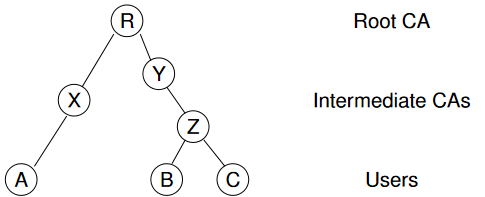
\includegraphics[scale=0.7]{Images/hierarchicalpki.png}
\label{fig:fround}
\caption{Hierarchical PKI.}
\end{figure}

CAs certify the public key of the entity below.

\subsubsection{Revocation}

Sometimes it may be required to declare a certificate invalid even though its validity period is current.\\
In order to make this work the user must check to see which certificates have been revoked.\\
Two widely deployed mechanisms:
\begin{enumerate}
    \item Certificate revocation lists (CRL): each CA periodically issues a list of revoked certificates which can be downloaded and then checked by clients.
    \item Online certificate status protocol (OCSP): a server will maintain a current list of revoked certificates and respond to requests about specific certificates.
\end{enumerate}

\newpage \section{Protocols for Key Establishment}

\subsection{Principles}

\subsubsection{Types of keys}

\begin{itemize}
    \item Long term keys (static keys): intended to be used for long period (few hours $\rightarrow$ few years). Symmetric or asymmetric, depends on how they're used.
    \item Ephemeral keys: generated for single use and then deleted.
    \item Session keys: intended for use in one communication session (few seconds, few hours or a day), to protect communications in a session for example with authenticated encryption. Usually symmetric keys used with ciphers such as AES and MACs because of their better efficiency over public key algorithms.
\end{itemize}
Long-term and ephemeral keys are used in establishment of sessions keys.

\subsubsection{Key establishment}

We need way to establish secret session keys among communication parties using long-term keys. 3 approaches:
\begin{enumerate}
    \item key pre-distribution where keys are set in advance
    \item key transport where one party chooses the key and distributes it
    \item key agreement where 2+ parties contribute to the session key.
\end{enumerate}

\subsubsection{Security}

Adversary capabilities: we assume attacker can eavesdrop on all messages, alter all messages, re-route any message to any user, obtain the value of the session key $K_{AB}$ used in any previous run of the protocol.

2 properties define security:
\begin{itemize}
    \item Authentication: if party $A$ completes the protocol and believes that sessions key $K_{AB}$ is shared with party $B$, then $K_{AB}$ should not be shared with a different party $C$.\\
    Can be mutual (both parties achieve it) or unilateral ( only provided on one side).
    \item Confidentiality: an adversary is unable to obtain the session key accepted by a particular party.
\end{itemize}

(Perfect) forward secrecy: compromise of long-term private keys does not reveal session keys previously agreed using those long-term keys.

\subsection{Types}

\subsubsection{Key pre-distribution (pre-shared keys)}

Trusted authority (TA) generates and distributes long-term keys to all users when they join the system.\\
Simplest scheme: secret key for each pair (poor scalability). More complex schemes give each user a set of keys so that each pair has a subset.

\subsubsection{Session key transport with an online server}

TA shares a long-term shared key with each user.\\
TA generates and sends session keys to users when requested and protected by the long-term keys.\\
Example: Kerberos (see \ref{Kerberos}).\\
TA must be trusted and is single point of attack + problems of scalability.

\subsubsection{Key transport with asymmetric cryptography}

One user chooses key material and sends it encrypted with the other party's public key.\\
TLS up to 1.2 includes options for this type of key establishment.\\
No forward secrecy.

\subsubsection{Key agreement - signed Diffie-Hellman}

2 parties each provide input to the keying material.\\
Usually provide authentication with public keys, for example by signing the exchanged messages.\\
Diffie–Hellman protocol is a widely used key agreement protocol.\\
TLS includes options for this type of key distribution.

\textbf{Signed Diffie-Hellman}

$A$ and $B$ are two parties with identities $ID_A$, $ID_B$, who want to share a session key.\\
Computation takes place in a group $G$ with generator $g$ .\\
$a, b$ are random values chosen by $A$ and $B$ in the range up to the order of $G$.\\
$Sig_A(m)$ is a digital signature on message $m$ by $A$.\\
$Sig_B(m)$ is a digital signature on message $m$ by $B$.\\
Both parties need each other’s public signature verification keys.\\
Provides forward secrecy because the long-term (signing) keys are only used for authentication.

\begin{figure}[H]
\centering
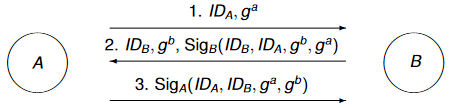
\includegraphics[scale=0.75]{Images/signeddiffiehellmanprotocol.png}
\label{fig:fround}
\caption{Signed Diffie-Hellman protocol.}
\end{figure}

$A$ checks the signature received in flow 2 and if it is valid $A$ computes the shared secret : $Z= (g^b)^a=g^{ab}$.\\
Similarly $B$ checks the signature received in flow 3 and, if valid, computes the shared secret: Z=  $Z= (g^b)^a=g^{ab}$.\\
The session key can be $K_{AB}=H(Z,ID_A,ID_B)$.

\subsection{Session key transport using symmetric keys}

\subsubsection{Needham-Schroeder protocol}

\textbf{Protocol}

\noindent\begin{minipage}{0.6\textwidth}% adapt widths of minipages to your needs
\begin{figure}[H]
\centering
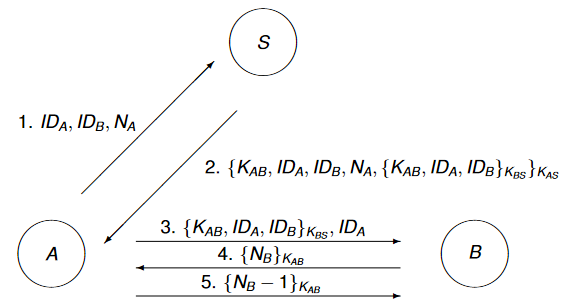
\includegraphics[scale=0.7]{Images/needhamschroederprotocol.png}
\label{fig:fround}
\caption{Needham-Schroeder protocol.}
\end{figure}
\end{minipage}%
\hfill%
\begin{minipage}{0.35\textwidth}
\begin{itemize}
    \item Parties $A, B$ want to establish session key.
    \item Party $S$ is the TA
    \item $A$ and $S$ share long-term key $K_{AS}$.
    \item $B$ and $S$ share long-term key $K_{BS}$.
    \item $K_{AS}$: new session key generated by $S$.
    \item Nonces $N_A, N_B$ randomly generated for one-time use.
    \item $\{X\}_K$: authenticated encryption of message $X$ using shared secret key $K$.
\end{itemize}
\end{minipage}

\textbf{Replay attack}

An attacker is able to replay old protocol messages and the honest party accepts an old session key.\\
Assume an attacker $C$ obtains a sessions key $K'_{AB}$ previously established between $A$ and $B$.\\
In the attack, $C$ masquerades as $A$ and is thus able to persuade $B$ to use the old key $K'_{AB}$.

\begin{figure}[H]
\centering
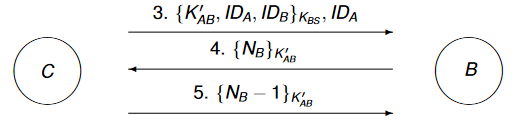
\includegraphics[scale=0.7]{Images/replayattackneedham.png}
\label{fig:fround}
\caption{Replay attack on Needham-Schroeder protocol.}
\end{figure}

\textbf{Repaired Needham-Schroeder protocol: freshness}

To defend against replay attacks: critical that the key established be fresh (new) for each session.\\
To achieve freshness: random challenges (nonces), timestamps (string on the current time), counters (increased for each new message).
Example with random challenges:

\begin{figure}[H]
\centering
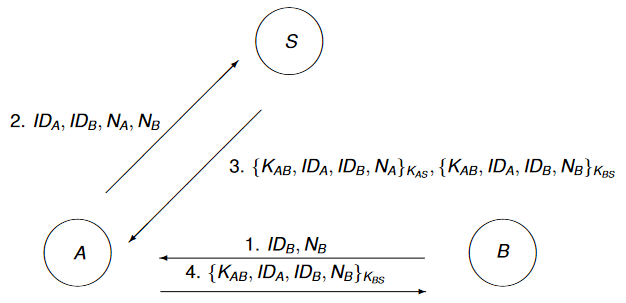
\includegraphics[scale=0.7]{Images/reparedneedhamschroeder.png}
\label{fig:fround}
\caption{Repaired Needham-Schroeder protocol - use of random challenges.}
\end{figure}

\textbf{Repaired Needham-Schroeder protocol: tickets}

Use of key with validity period to fix protocol.\\
\noindent\begin{minipage}{0.6\textwidth}% adapt widths of minipages to your needs
\begin{figure}[H]
\centering
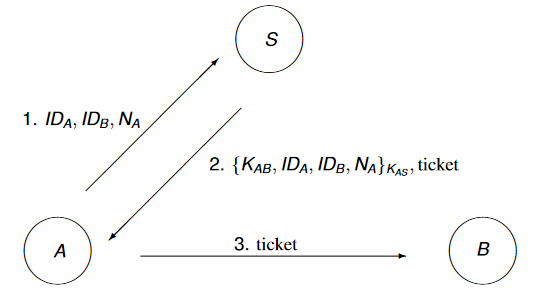
\includegraphics[scale=0.72]{Images/needhamschroedertickets.png}
\label{fig:fround}
\caption{Repaired Needham-Schroeder protocol - use of tickets.}
\end{figure}
\end{minipage}%
\hfill%
\begin{minipage}{0.35\textwidth}
\begin{itemize}
    \item Suppose $A$ wants to obtain access to server $B$.
    \item Authentication server$S$ issues a ticket to allow $A$ to obtain access.
    \item Ticket has the format $\{K_{AB}, ID_A, ID_B, T_B\}_{K_{BS}}$ where $T_B$ is a timestamp which we can also interpret as a validity period.
    \item $A$ can obtain the ticket and use it to gain access to $B$ at any time while $T_B$ is valid.
\end{itemize}
\end{minipage}

\subsubsection{Kerberos}\label{Kerberos}

Since Windows 2000, Kerberos V5 is the default Windows domain authentication method. \\
A single sign-on (SSO) solution: users only need to enterusernames and passwords once for a session.\\
Provide access selectively for a number of different online services using individual tickets. Establish session key to deliver confidentiality and integrity services for each service access.

\textbf{Three level protocol}

\begin{itemize}
    \item Level 1: Client $C$ interacts with authentication server $AS$ in order to obtain a ticket-granting ticket – happens once for a session (maybe a working day)
    \item Level 2: Client $C$ interacts with ticket-granting server $TGS$ in order to obtain a service ticket – happens once for each server during the session
    \item Level 3: Client $C$ interacts with application server $V$ in order to obtain a service – happens each time the client requires service during the session
\end{itemize}

\textbf{Level 1: interaction with authentication server}

\noindent\begin{minipage}{0.6\textwidth}% adapt widths of minipages to your needs
\begin{figure}[H]
\centering
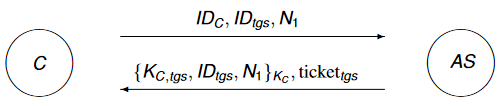
\includegraphics[scale=0.72]{Images/kerberoslevel1.png}
\label{fig:fround}
\caption{Kerberos level 1 - interaction with authentication server.}
\end{figure}
\end{minipage}%
\hfill%
\begin{minipage}{0.35\textwidth}
\begin{itemize}
    \item $ticket_{tgs}=\{K_{C,tgs},ID_C,T_1\}_{K_{tgs}}$  for some validity period $T_1$
    \item Result: user has ticket-granting ticket which can be used to obtain different service-granting tickets.
\end{itemize}
\end{minipage}
\begin{itemize}
    \item $K_C$: symmetric key shared with authentication server $AS$ (typically generated by the workstation of $C$ from a password entered by $C$ at logon time)
    \item $K_{C,tgs}$: new symmetric key generated by $AS$ to share with the ticket-granting server $TGS$
    \item $N_1$: nonce used by $C$ to check that $K_{C,tgs}$ is fresh
    \item $K_{tgs}$: long-term key shared between $AS$ and $TGS$.
\end{itemize}

\textbf{Level 2: interaction with ticket-granting server}

\noindent\begin{minipage}{0.6\textwidth}% adapt widths of minipages to your needs
\begin{figure}[H]
\centering
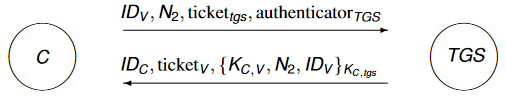
\includegraphics[scale=0.72]{Images/kerberoslevel2.png}
\label{fig:fround}
\caption{Kerberos level 2 - interaction with ticket-granting server.}
\end{figure}
\end{minipage}%
\hfill%
\begin{minipage}{0.38\textwidth}
\begin{itemize}
    \item $ticket_{V}=\{K_{C,V},ID_C,T_2\}_{K_{V}}$  for some validity period $T_2$
    \item $authenticator_{TGS}=\{ID_C,TS_1\}_{K_{C,tgs}}$  for some timestamp $TS_1$
    \item Result: user has service-granting ticket which can be used to obtain access to a specific server.
\end{itemize}
\end{minipage}
\begin{itemize}
    \item $ticket_{tgs}$: same as sent in level 1
    \item $K_{C,V}$: session key to be used with server $V$ 
    \item $N_2$: nonce used by $C$ to check that $K_{C,V}$ is fresh
    \item $TGS$ first obtains $K_{C,tgs}$ from $ticket_{tgs}$ and then checks if the fields in the authenticator are valid – includes checking that $TS_1$ is recent and that $C$ is authorized to access service $V$
    \item $AS$ and $TGS$ may be the same machine.
\end{itemize}

\textbf{Level 3: interaction with application server}

\noindent\begin{minipage}{0.6\textwidth}% adapt widths of minipages to your needs
\begin{figure}[H]
\centering
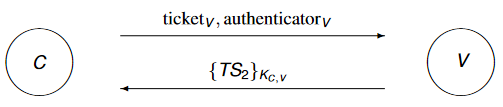
\includegraphics[scale=0.72]{Images/kerberoslevel3.png}
\label{fig:fround}
\caption{Kerberos level 3 - interaction with application server.}
\end{figure}
\end{minipage}%
\hfill%
\begin{minipage}{0.38\textwidth}
\begin{itemize}
    \item $authenticator_{V}=\{ID_C,TS_2\}_{K_{C,V}}$  for some timestamp $TS_2$
    \item Result: user has secure access to specific server $V$.
\end{itemize}
\end{minipage}
\begin{itemize}
    \item $ticket_{V}$: same as sent in level 2
    \item $K_{C,V}$ is contained in $ticket_V$ and was also sent to $C$ in the level 2 interaction
    \item The reply from $V$ is intended to provide mutual authentication so that $C$ can check it is using the right service $V$.
\end{itemize}

\textbf{Limitations}

Limited scalability: even though different realms are supported, each realm needs to share a key with each other realm.\\
Suited for corporate environments with shared trust (although public key variants exist).\\
Offline password guessing is a possible attack when the client key $K_C$is derived from a human memorable password.\\
Kerberos standard does not specify how to use the session key once it is established.

\newpage
\section{Transport Layer Security (TLS) Protocol}

\subsection{Overview}

Most widely used security protocol. Used to secure communications with banks, online shops, ...\\
TLS 1.2 is currently the most popular version. For TLS 1.3 see \ref{TLS1.3}.\\
Often used to allow browsers to establish secure sessions with web servers.\\
Runs primarly over TCP - variant DTLS runs over datagram protocols.

\subsubsection{Architecture}

\noindent\begin{minipage}{0.54\textwidth}% adapt widths of minipages to your needs
\begin{figure}[H]
\centering
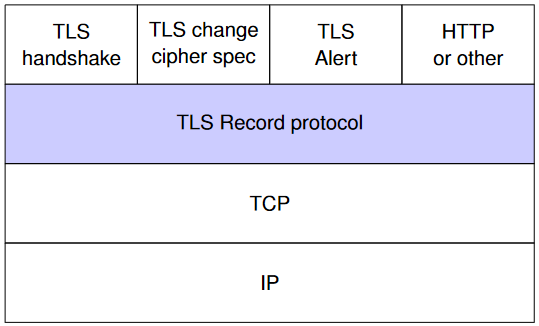
\includegraphics[scale=0.55]{Images/tlsprotocolstack.png}
\label{fig:fround}
\caption{TLS protocol stack.}
\end{figure}
\end{minipage}%
\hfill%
\begin{minipage}{0.55\textwidth}
3 higher level protocols:
\begin{itemize}
    \item TLS handshake protocol: set up sessions
    \item TLS alert protocol: signal events (3 types of alerts: warning alerts, 'close\_notify' alerts, fatal alerts). Improper handling of alert messages can lead to truncation attacks.
    \item TLS change cipher spec protocol: change cryptographic algorithms. Normally used after the handshake protocol to indicate commencement of secure traffic.
\end{itemize}
\end{minipage}

\subsubsection{TLS ciphersuites}

Specify the public key algorithms used in the handshake protocol and the symmetric algorithms used in the record protocol.\\
> 300 standardized suites, many weak and should not be used.\\
Example: TLS\_RSA\_WITH\_3DES\_EDE\_CBC\_SHA.

Common TLS 1.2 ciphersuites:
\begin{itemize}
    \item Handshake algorithm (all use signed Diffie-Hellman):
    \begin{itemize}
        \item DHA-RSA: Ephemeral Siffie-Hellman with RSA signatures
        \item ECDHE-RSA: Elliptic curve DHE with RSA signatures
        \item DHE-DSS: DHE with DSS signatures
    \end{itemize}
    \item Record algorithms:
    \begin{itemize}
        \item AES-GCM: AES authenticated encryption with GCM mode
        \item AES-CBC-SHA256: AES in CBC mode with HMAC from SHA256
        \item CHACHA20-POLY1305: ChaCha stream cipher with Poly1305 MAC
    \end{itemize}
\end{itemize}

\subsection{TLS Record Protocol}

Provides 2 services: message confidentiality and message integrity.\\
Services can be provided by symmetric encryption and a MAC.\\
For TLS1.2+, theses services are often provided with authenticated encryption with associated data (AEAD) modes CCM or GCM.\\
The handshake protocol establishes symmetric keys(session keys) to use with these mechanisms.

\noindent\begin{minipage}{0.54\textwidth}% adapt widths of minipages to your needs
\begin{figure}[H]
\begin{center}
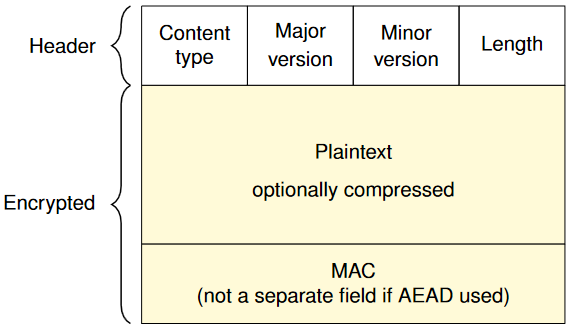
\includegraphics[scale=0.55]{Images/tlsrecordprotocolformat.png}
\label{fig:fround}
\caption{TLS record protocol format.}
\end{center}
\end{figure}
\end{minipage}%
\hfill%
\begin{minipage}{0.42\textwidth}
Record protocol header:
\begin{itemize}
    \item Content type: types are change-cipher-spec, alert, handshake, application-data
    \item Protocol version: major version (3 for TLS), minor version (1 for TLS v1.0, 2 for v1.1, 3 for v1.2)
    \item Length: length in octets of the data.
\end{itemize}
\end{minipage}

\subsubsection{Record protocol operation}

Fragmentation: Each application layer message is fragmented into blocks of 214 bytes or less.\\
Compression: Optionally applied – default compression algorithm is null.\\
Authenticated data: consists of the (compressed) data, the header, and an implicit record sequence number.\\
Plaintext: Compressed data and the MAC, if present.\\
Session keys for the MAC and encryption algorithms, or AEAD algorithm, are established during the handshake protocol.\\
The encryption and MAC algorithms are specified in the negotiated ciphersuite.

\subsubsection{Cryptographic algorithms}

\begin{itemize}
    \item MAC:  The algorithm used is HMAC in all TLS versions using a negotiated hash function. SHA-2 is allowed only from TLS 1.2.
    \item Encryption:  Either a negotiated block cipher in CBC mode or a stream cipher. Most common block ciphers are AES and 3DES. RC4 originally supported in TLS1.2. For block ciphers, padding is applied after the MAC to make a multiple of the cipher block size.
    \item AEAD:  Allowed instead of encryption and MAC in TLS1.2. Usually AES in CCM or GCM modes. Authenticated additional data is the header and implicit record sequence number.
\end{itemize}

\subsection{TLS Handshake Protocol}

Negotiates the version of TLS and the cryptographic algorithms to be used.\\
Establishes a shared session key for use in the record protocol.\\
Authenticates the server. Authenticates the client (optional).\\
Completes the session establishment.\\
Several variations of the handshake: IRSA variant (still supported but not recommended), Diffie-Hellman variant (recommended), Pre-shared key variant, Mutual authentication or server-only authentication.

\subsubsection{Four phases}

\noindent\begin{minipage}{0.54\textwidth}% adapt widths of minipages to your needs
\begin{figure}[H]
\begin{center}
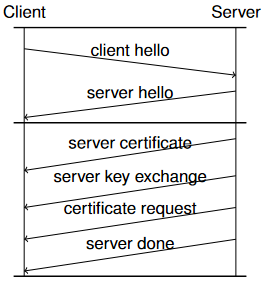
\includegraphics[scale=0.7]{Images/tlshandshakephase12.png}
\label{fig:fround}
\end{center}
\end{figure}
\end{minipage}%
\hfill%
\begin{minipage}{0.42\textwidth}
\begin{itemize}
    \item Phase 1: Client and server negotiation version, cipher suite and compression and exchange nonces.
    \item Phase 2: Server sends certificate and key exchange message (if needed).
\end{itemize}
\end{minipage}

\noindent\begin{minipage}{0.54\textwidth}% adapt widths of minipages to your needs
\begin{figure}[H]
\begin{center}
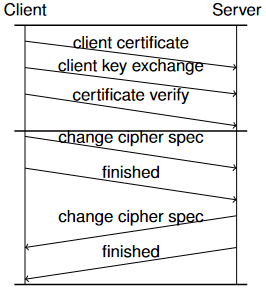
\includegraphics[scale=0.7]{Images/tlshandshakephase34.png}
\label{fig:fround}
\end{center}
\end{figure}
\end{minipage}%
\hfill%
\begin{minipage}{0.42\textwidth}
\begin{itemize}
    \item Phase 3: Client sends certificate and key exchange message.
    \item Phase 4: Client and server start secure communications.
\end{itemize}
Finished messages include a check value (pseudo-random function) of all the previous messages.
\end{minipage}

Main messages:
\begin{itemize}
    \item Client hello: States highest version of TLS available, advertises ciphersuites available to the client and sends client nonce $N_C$.
    \item Server hello: Returns the selected version and ciphersuite and sends server nonce $N_S$ 
    \item Server key exchange: Server’s input to key exchange.
    \item Client key exchange: Client input to key exchange.
    \item Change-cipher-spec: Switch to newly negotiated ciphersuite for record .
\end{itemize}

\textbf{Generating session keys}

The master secret $ms$ is defined using the premaster secret $pms$: $ms=PRF(pms,“master secret”,N_C\Vert N_S)$.\\
As much keying material is generated as is required by the ciphersuite using: $k=PRF(ms,“key expansion”,N_S\Vert N_C)$.\\
Independent session keys are partitioned from $k$ in each direction (a write key and a read key on each side).\\
Depending on ciphersuite, keying material may include: encryption key, MAC key, IV.

\textbf{Pseudorandom function PRF}

The PRF (pseudo-random function) is built from HMAC with a specified hash function: in TLS 1.0 and 1.1 based on a combination of MD5 and SHA-1; in TLS 1.2  based on SHA-2.\\
For example, in TLS 1.2: $PRF(K,label,r)  =HMAC(K,A(1) \Vert label \Vert r) \Vert HMAC(K,A(2)\Vert label \Vert r)\Vert...$ where $A(0) =r, A(i) =HMAC(K,A(i−1))$ and HMAC uses a specified SHA-2 variant, typically SHA256, as its hash function.

\subsubsection{Handshake variants}

\textbf{Ephemeral Diffie–Hellman handshake variant}

Server key exchange: Diffie–Hellman generator and group parameters and server ephemeral Diffie-Hellman value, all signed by server.\\
Client key exchange: Client ephemeral Diffie-Hellman value. This is optionally signed by the client if the client certificate is used.\\
Pre-master secret $pms$ is the shared Diffie–Hellman secret.\\
Provides forward secrecy and therefore recommended today.

\textbf{RSA Handshake variant}

Server key exchange: Not used.\\
Client key exchange: Key transport of pre-master secret $pms$. Client selects a random pre-master secret $pms$. Client encrypts $pms$ with the server’s public key and sends the ciphertext to the server. Server decrypts using its private key to recover $pms$.\\
No forward secrecy and NOT recommended today.

\textbf{Diffie-Hellman (DH)}

The parties use static Diffie–Hellman with certified keys — if the client does not have a certificate (usual on the Internet) then the client uses an ephemeral Diffie-Hellman key.

\textbf{Anonymous Diffie-Hellman (DH\_Anon)}

The ephemeral Diffie-Hellman keys are not signed at all, so only protects against passive eavesdropping.

\subsection{Attacks}

\subsubsection{TLS limitations}

Many servers do not support the latest version of TLS and/or have not protected against known attacks.\\
\href{https://www.ssllabs.com/ssl-pulse/}{SSL Pulse Survey} gives an up-to-date picture of current attacks.

\subsubsection{BEAST}

Browser Exploit Against SSL/TLS: exploits non-standard use of IV in CBC mode encryption - IVs are chained from previous ciphertexts.\\
Allows attacker to recover plaintext byte by byte.\\
From TLS 1.1 only random IV is allowed.\\
Mitigation strategy (implemented in most browsers): splitting plaintext into first byte + remainder to force a randomised IV including a MAC computation.\\
No longer considered a realistic threat.

\subsubsection{CRIME and BREACH}

Side channel attacks base on compression - different inputs result in different amounts of compression.\\
CRIME (Compression Ratio Info-leak Made Easy) exploits compression in TLS, while BREACH (Browser Reconnaissance and Exfiltration via Adaptive Compression of Hypertext) exploits compression in HTTP.\\
Commonly recommended to switch off compression in TLS but switching off in HTTP too results in big performance penalty.

\subsubsection{Padding oracles and POODLE}

A padding oracle is a way for an attacker to know if a message in a ciphertext was correctly padded. Shown how in theory CBC mode encryption can provide a padding oracle due to its error propagation properties.\\
POODLE (Padding Oracle On Downgraded Legacy Encryption) published in October 2014 forces downgrade to SSL 3.0 and then runs padding oracle attack.\\
Main mitigation: uniform error response, so that the attacker cannot distinguish padding errors from MAC errors.

\subsubsection{Heartbleed bug}

An implementation error in OpenSSL. Based on missing bounds check in heartbeat messages.\\
Allows memory leakage from server which is likely to include session keys and long-term keys.

\subsubsection{Man-in-the-middle}

MITM attacks: rely on issuing a new certificate and installing a root certificate in the browser.

\newpage
\section{TLS 1.3}\label{TLS1.3}

TLS 1.3 is the latest version of the Transport Layer Security protocol and has significant changes from earlier versions affecting both security and efficency.

\subsection{Development - Why was TLS 1.3 needed ?}

Efficiency: TLS1.2- nneds at least 2 round trip times (RTT) before data can be sent.\\
Security: problems in earlier version (too complex, support of old/weak ciphersuites).

\subsection{Differences}

\subsubsection{Protocols}

Handshake: similar purpose but fewer rounds.\\
Record: similar to TLS 1.2.\\
Alert: similar to TLS 1.2.\\
No TLS change cipher spec protocol.

\subsubsection{Some changes}

\noindent\begin{minipage}{0.48\textwidth}% adapt widths of minipages to your needs
Some items removed:
\begin{itemize}
    \item static RSA and DH key exchange
    \item renegotiation
    \item SSL 3.0 negotiation
    \item DSA in finite fields
    \item data compression
    \item non-AEAD cipher suites
\end{itemize}
\end{minipage}%
\hfill%
\begin{minipage}{0.48\textwidth}
Some items added:
\begin{itemize}
    \item encrypted content type
    \item 0-RTT mode (from pre-shared key)
    \item post-handshake client authentication through 'certificate verify' signature
    \item more AEAD ciphersuites
\end{itemize}
\end{minipage}

\subsubsection{TLS 1.3 handshake protocol}

\textbf{Hello messages}
Client sends (optimistic) keyshare field in client hello for one or more anticipated ciphersuites.\\
Server can obtain session key on receipt of client hello if: server accepts one of the clients ciphersuites, client keyshare matches the accepted ciphersuite.\\
If the above conditions fail then: server sends an optional Hello Retry Request, client responds if there is an acceptable alternative ciphersuite.\\
Usually this results in saving a whole round trip of communication.

\textbf{Other messages}

Only client and server hello/keyshare messages are not cryptographically protected.\\
Key calculation uses standard HKDF (hash key derivation function) to derive the individual keys.\\
Several different key types derived from master secret: 'handshake traffic keys' to protect handshake protocol, 'application traffic keys' for client-server traffic, 'early data keys' for 0-RTT data.

\textbf{TLS 1.2 comparison}

\begin{figure}[H]
\begin{center}
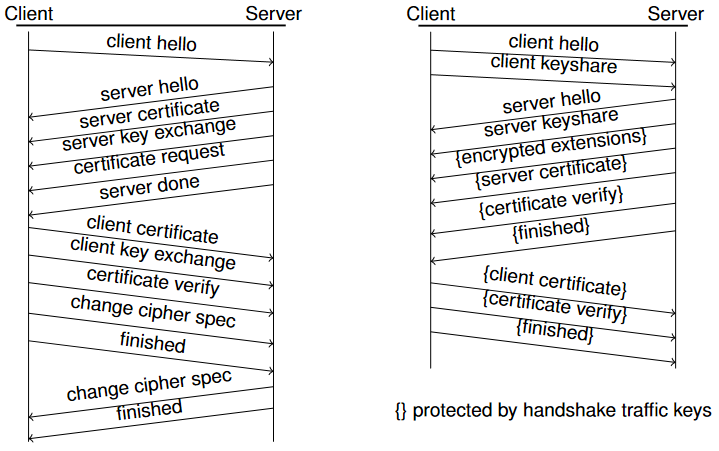
\includegraphics[scale=0.7]{Images/handshakecomparison.png}
\label{fig:fround}
\caption{Handshake comparison - TLS 1.2 to TLS 1.3}
\end{center}
\end{figure}

\subsubsection{Client authentication}

In TLS 1.2 and 1.3 it is optional for the client to send a certificate and authenticate using a 'CertificateVerify' message. The 'CertificateVerify' message includes a signature which can be verified using the public key in the certificate.\\
TLS 1.3 adds a 'post-handshake client authentication' extension; if this is used then the server may request client authentication at any time after the handshake completed. The client responds with its certificate and a signature in the form of 'CertificateVerify'.

\subsubsection{0-RTT in TLS 1.3}

\noindent\begin{minipage}{0.48\textwidth}% adapt widths of minipages to your needs
\begin{figure}[H]
\begin{center}
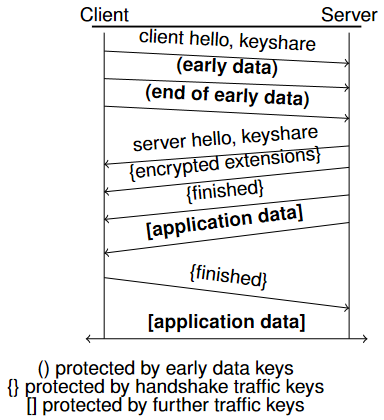
\includegraphics[scale=0.58]{Images/0rtttls13.png}
\label{fig:fround}
\caption{0-RTT in TLS 1.3.}
\end{center}
\end{figure}
\end{minipage}%
\hfill%
\begin{minipage}{0.48\textwidth}
\begin{itemize}
    \item In a 0-RTT key establishment parties can start sending application data immediately, so-called early data
    \item Based on pre-shared key (PSK)
    \item PSK can either be agreed outside TLS or from an earlier TLS session
    \item At the end of the handshake protocol the server can send to the client one or more new session tickets as PSKs
    \item A client may start a new PSK session without negotiating version and ciphersuite.
\end{itemize}
\end{minipage}

\subsubsection{Ciphersuites}

Same cipher suite coding as previous versions.\\
TLS 1.2 and lower cipher suite values cannot be used with TLS 1.3 and vice versa.\\
Handshake always uses Diffie-Hellman option so (ECDHE) not explicitly stated.\\
Mandatory to implement ciphersuite: TLS\_AES\_128\_GCM\_SHA256.\\
Recommended ciphersuites: TLS\_AES\_256\_GCM\_SHA384, TLS\_CHACHA20\_POLY1305\_SHA256, TLS\_AES\_128\_CCM\_SHA256, TLS\_AES\_128\_CCM\_8\_SHA256.

\subsubsection{ChaCha algorithm}

Stream cipher defined in RFC 8439 together with a message authentication code (MAC) called Poly1305.\\
Faster than AES, except for processors with AES hardware support (most modern desktop computers).\\
Combines $\oplus$, addition modulo $2^32$ and rotation operations over 20 rounds to produce 512 bits of keystream.\\
256-bit key.

\subsubsection{Main improvements}

\begin{itemize}
    \item Efficiency:
    \begin{itemize}
        \item Saving of one RTT in handshake
        \item Can set up follow-up session with 0-RTT
    \end{itemize}
    \item Security:
    \begin{itemize}
        \item Only forward-secret key exchange allowed
        \item Many legacy ciphersuites no longer allowed
        \item Renegotiation option removed
        \item Formal security proofs
    \end{itemize}
\end{itemize}

\subsubsection{Selfie attack}

Published 2019.\\
Breaks mutual authentication in PSK mode.\\
Victim party Alice must be prepared to act as a client and a server.\\
Suppose Alice shares a PSK with Bob.\\
Attacker reflects messages back to herself so client Alice believes she is talking to Bob while she is actually talking with server Alice.\\
Case is not covered in formal analysis of TLS 1.3.\\
Can be prevented by forbidding to share PSK between more than one server and one client.

\newpage
\section{IP Layer Security (IPsec)}

Provides protection for any higher layer protocol, including arbitrary TCP and UDP sessions.\\
Uses encryption, authentication and key management algorithms.\\
Most commonly used to provide Virtual Private Networks(VPNs).\\
Provides a security architecture for both IPv4 and IPv6.

\subsection{Security services}

\begin{itemize}
    \item Message confidentiality: Protects against unauthorised data disclosure by the use of encryption.
    \item Message integrity: Detects if data has been changed by using a message authentication code (MAC) or authenticated encryption.
    \item Limited traffic analysis protection: Eavesdropper on network traffic should not know which parties communicate, how often, or how much data is sent.
    \item Message replay protection: The same data is not replayed and data is not delivered badly out of order.
    \item Peer authentication: Each IPsec endpoint confirms the identity of the other IPsec endpoint.
\end{itemize}

\subsection{Architectures}

\subsubsection{Gateway-to-gateway}

Provides secure network communications between 2 networks.\\
Network traffic is routed through the IPsec connection, protecting it appropriately.\\
Only protects data between the two gateways.\\
Most often used when connecting two secured networks, such as linking a branch office to headquarters over the Internet.\\
Can be less costly than private wide area network (WAN) circuits.

\subsubsection{Host-to-gateway}

Commonly used to provide secure remote access.\\
The organization deploys a virtual private network (VPN) gateway onto their network.\\
Each remote access user establishes a VPN connection between the local computer (host) and the gateway.\\
VPN gateway may be a dedicated device or part of another network device.\\
Most often used when connecting hosts on unsecured networks to resources on secured networks.

\subsubsection{Host-to-host}

Typically used for special purpose needs, such as system administrators performing remote management of a single server.\\
Only model that provides protection for data throughout its transit (end-to-end).\\
Resource-intensive to implement and maintain in terms of user and host management.\\
All user systems and servers that will participate in VPNs need to have VPN software installed and/or configured.\\
Key management is often accomplished through a manual process.

\subsection{Protocols}

\subsubsection{Types}

\begin{itemize}
    \item Encapsulating Security Payload (ESP): Can provide confidentiality, authentication, integrity and replay protection.
    \item Authentication Header (AH): Authentication, integrity and replay protection, but no confidentiality and is now deprecated.
    \item Internet Key Exchange (IKE): negotiate, create, and manage session keys in so-called 'security associations'.
\end{itemize}

\subsubsection{Setting up IsPsec connection}

Key exchange uses IKEv2 protocol (uses Diffie-Hellman protocol authenticated with public keys in X.509 certificates).\\
Includes 'cookies' to mitigate denial-of-service attacks: client must return a time-dependent cookie value before the server proceeds; they provide proof of reachability before any expensive cryptographic processing is completed.

\subsubsection{Security associations}

A security association (SA) contains info needed by an IPsec endpoint to support an IPSec connection.\\
Can include cryptographic keys and algorithms, key lifetimes, security parameter index (SPI), and security protocol identifier (ESP or AH).\\
SPI is included in the IPSec header to associate a packet with the appropriate SA.\\
SA tells the endpoint how to process inbound IPSec packets or how to generate outbound packets.\\
SAs are needed for each direction of connection.\\
IKEv2 is used to establish keys to use in SAs.

\subsubsection{Cryptographic suites}

Similar to TLS ciphersuites: standardised suites (both public key and symmetric key algorithms).\\
Specific groups available for Diffie-Hellman, both in finite fields and on elliptic curves.\\
3DES or AES can be used for encryption, either in CBC or GCM.\\
HMAC or CMAC (variant) is used for integrity if GCM mode is not used.

\subsection{Modes}

Each protocol (ESP or AH) can operate in transport or tunnel mode.
\begin{itemize}
    \item Transport mode: Maintains IP header of the original packet and protects payload — generally only used in host-to-host architectures.
    \item Tunnel mode: Original packet encapsulated into a new one, payload is original packet — typical use is gateway-to-gateway architecture
\end{itemize}
We show the pictures for IPv4 — there are slight differences for IPv6.

\subsubsection{Protocol components}

\begin{itemize}
    \item ESP header: contains security parameter index (SPI) identifying the SA and sequence numbers
    \item ESP trailer: contains padding and padding length - may also include extra padding to enhance traffic flow confidentiality
    \item ESP Auth: contains MAC of the encrypted data and ESP header - may not be required if an authenticated encryption mode is used.
\end{itemize}

\subsubsection{Transport mode ESP}

Original IP packet:
\begin{center}
\begin{tabular}{ | c | c | }
\hline
IP header & Data
\end{tabular}
\end{center}
IP packet protected by Transport-ESP:
\begin{figure}[H]
\begin{center}
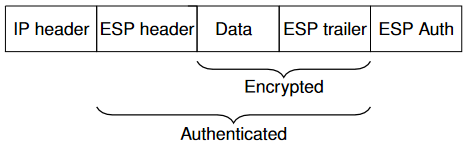
\includegraphics[scale=0.58]{Images/ippackettransportesp.png}
\label{fig:fround}
\end{center}
\end{figure}

Data after the original IP header is padded by adding an ESP trailer and result encrypted using the symmetric cipher and key in the SA.\\
An ESP header is prepended.\\
If an SA uses the authentication service, an ESP MAC is calculated over the data prepared so far and appended.\\
Original IP header is prepended, but some fields in the original IP header must be changed: protocol field changes from TCP to ESP, total length field must be changed to reflect the addition of the ESP header, checksums must be recalculated.

\subsubsection{Tunnel mode ESP}

Original IP packet:
\begin{center}
\begin{tabular}{ | c | c | }
\hline
IP header & Data
\end{tabular}
\end{center}
IP packet protected by Tunnel-ESP:
\begin{figure}[H]
\begin{center}
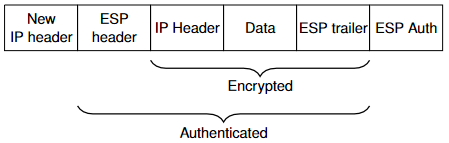
\includegraphics[scale=0.58]{Images/ippackettunnelesp.png}
\label{fig:fround}
\end{center}
\end{figure}

Entire original packet is padded by adding an ESP trailer and the result encrypted using the symmetric cipher and key agreed in the SA.\\
ESP header is prepended.\\
If the SA uses the authentication service, an ESP MAC is calculated over the data prepared so far and appended.\\
New outer IP header is prepended.\\
Inner IP header of the original IP packet carries the ultimate source and destination addresses.\\
Outer IP header may contain distinct IP addresses such as addresses of security gateways.\\
Outer IP header protocol field is set to ESP.

\subsection{Security}

Active attacks have been demonstrated for encryption-onlymode of ESP protocol — now widely understood that providing encryption without integrity is insecure.\\
Unlike earlier versions of IPsec, the 2005 version does not require implementations to support encryption-only mode, but still allows it.\\
ESP applies encryption before MAC in normal usage.\\
Using AH, a MAC can be applied before encryption, as in TLS. Attacks have been demonstrated on such configurations.\\
Formal analysis has shown that IPsec key exchange protocol (IKEv2) has no significant weaknesses.

\newpage
\section{Email Security and Secure Messaging}

\subsection{Email Security Requirements}

\subsubsection{Email architecture}

Message user agent (MUA) connects client to mail system. Uses SMTP to send mail to message submission agent(MSA) and POP or IMAP to retrieve mail from message store (MS).\\
Message handling system (MHS) transfers message from MSA to MS via one or more message transfer agent (MTA).\\
Simple message transfer protocol (SMTP) is mail transmission protocol defined in RFC 5321.

\subsubsection{Threats}

Usual 'CIA' categories.\\
Content may require confidentiality/authentication.\\
Availability of the email service may be threatened.\\
Metadata in header information is a significant source of attacker information.

\subsection{Email security}

\subsubsection{Link security}

\textbf{STARTTLS}

Extensions to mail protocols SMTP, POP and IMAP to run over TLS connections.\\
Provides link-by-link security, not end-to-end security.\\
Opportunistic use of TLS security (encryption) — use it if possible $\Rightarrow$ vulnerable to so-called STRIPTLS attacks – attacker interrupts TLS negotiation and connection falls back to plaintext transmission.\\
Defined for IMAP and POP3 (RFC 2595) and for SMTP (RFC 3207) amongst other protocols.\\
Widely used by prominent email providers including Gmail and Microsoft Outlook.

\textbf{DomainKeys Identified Mail (DKIM)}

Allows sending mail domain to sign outgoing mail using RSA signatures (currently supported signature algorithm).\\
Receiving domain can verify origin of mail.\\
Widely used by prominent email providers including Gmail.\\
Helps prevent email spoofing and hence reduce spam and phishing.\\
Public verification key of sending domain retrieved using DNS.

\begin{figure}[H]
\begin{center}
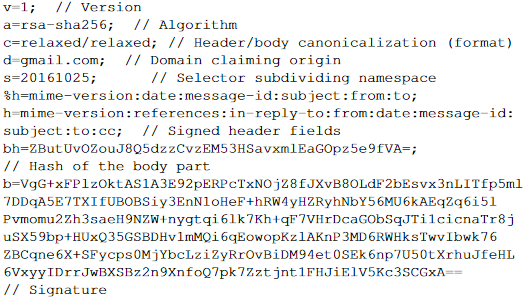
\includegraphics[scale=0.59]{Images/exampledkimsignature.png}
\label{fig:fround}
\caption{Example DKIM signature.}
\end{center}
\end{figure}

The ’d=’ and ’s=’ parts of the DKIM signature specify domain and selector.\\
The relevant public key is in the DNS record for the hostdefined by the host name: \texttt{[selector].\_domainkey.[domain]} where \texttt{s=} value is the selector and \texttt{d=} value is the domain.\\
In the example header above the nslookup would be: \texttt{nslookup -type=txt 20161025.\_domainkey.gmail.com}.

\subsubsection{End-to-end security}

\textbf{Email processing}

Protection of email message contents.\\
Hybrid encryption — a new random “session key” is generated for each object (message) and the session key is encrypted with the long-term public key of recipient.\\
Signing using RSA or DSA signatures.\\
Compression using Zip.\\
Coding using radix-64 to ensure that binary strings can be sent in email body.

\textbf{PGP encryption}

Session keys are encrypted using asymmetric encryption. OpenPGP requires support for ElGamal encryption and recommends also to support RSA encryption.\\
Encryption of message text using symmetric key encryption – OpenPGP requires support for 3DES with three keys (168 bits in total) and recommends also AES-128 and CAST5. Other algorithms are also defined.\\
Compression is applied before encryption.\\
Encryption can be applied independently of signing (no requirement for authenticated encryption).

\textbf{PGP signatures}

Plaintext message is optionally signed with sender’s private key.\\
OpenPGP standard requires support for RSA signatures.\\
DSA signatures also defined.\\
RSA signed messages are hashed with SHA1 (support required in standard) or other SHA2 hash functions.

\textbf{OpenPGP PKI}

Used in PGP email security.\\
Includes ID, public key, validity period and a self-signature.\\
No certification authorities — keys can be signed by anyone.\\
Various key servers used to store keys, such as \href{https://keys.openpgp.org/about}{https://keys.openpgp.org/about}.\\
Often known as the web of trust.\\
Autocrypt is an attempt to automate key management by including key information in the mail header — does not protect against active attacks.

\textbf{Problems with PGP}

Complicated for standard user to understand public key cryptography.\\
Typical problems: generating new keys securely, moving keys between devices, renewing keys.\\
Not available on iOS (although GnuPG exists now).\\
Outdated cryptographic algorithms still used: SHA1, CAST,Blowfish, ...\\
No support for SHA3 or authenticated encryption such as GCM.\\
A lot of metadata is available to an eavesdropper including: file length, encryption algorithm used, key identity of recipients.\\
No forward secrecy.\\
Does not support streaming mode or random access decryption.

\textbf{S/MIME}

Similar security features to PGP but different format for messages and not interoperable.\\
Requires X.509 format certificates instead of web of trust.\\
Supported natively by most popular mail clients.

\subsection{Secure Messaging}

\subsubsection{Differences with email}

Most instant messages are part of an interactive conversation with many messages over a long time.\\
Proprietary servers used to manage accounts.\\
Often (not necessarily) native applications are used.

\subsubsection{Security}

Standard CIA security services important as usual.\\
Forward secrecy: important especially for long sessions (use of 'medium-term' public keys stored at the server).\\
Post-compromise security (self-healing): an attacker who obtains a long-term key should b locked out again after communication resumes.

No 'standardized' security protocol.\\
Different ways to do:
\begin{itemize}
    \item Instagram, Snapchat, ...: no Ent-to-End encryption
    \item (Facebook) Messenger: no End-to-End by default
    \item iMessage, Whatsapp, Telegram are (allegedly) quite secure
    \item Signal Messenger is considered to be the best option.
\end{itemize}

\subsubsection{Signal protocol}

Signal server sets up initial authentication of user and registers initial public keys.\\
Public keys at the server are used to set up initial communication between users.\\
Key exchange uses elliptic curve Diffie–Hellman.\\
AES in CBC mode with HMAC (SHA256) used for message protection.\\
Protocol is used in Signal app and claimed also to be in WhatsApp and Facebook Messenger (closed source).

\textbf{Ratcheting}

A ratchet is a device which is easy to move forward but blocked from moving backward.\\
Signal uses a new unique message key for every message exchanged.\\
When successive messages sent in the same direction the message key is updated with a 'symmetric ratchet' by applying a function such as HMAC.\\
When a new message is returned in the opposite direction a new Diffie-Hellman ephemeral key is used to compute the new message key: this is the 'Diffie-Hellman ratchet'.\\
See \href{https://signal.org/docs/specifications/doubleratchet/}{https://signal.org/docs/specifications/doubleratchet/}

\subsubsection{Group messaging}

No good alternative for Diffie-Hellman is known in the multi-party case.\\
Signal uses a simple key distribution method for group messaging.\\
Currently a research effort is under way to develop Messaging Layer Security (mls) standard: \href{https://datatracker.ietf.org/wg/mls/about/}{https://datatracker.ietf.org/wg/mls/about/}.

% Inserting bibliography
\newpage
\pagenumbering{alph}
\printbibliography

% Inserting appendix with separate settings
%\addappendix
%\import{./Appendices/}{example_appendix}

% End of document
\end{document}
